\documentclass[journal]{IEEEtran}
\usepackage{amsmath,amssymb,booktabs,cite,graphicx,placeins}
\makeatletter\newcommand{\FigureContext}{\def\@captype{figure}}\makeatother
\usepackage[hidelinks]{hyperref}
\newif\ifnativecases
\ifdefined\NativeCaseReview\nativecasestrue\else\nativecasesfalse\fi
\newcommand{\CaseAsset}[2]{\ifnativecases local_figures/#2\else figures/journal_20261126/#1\fi}
\newcommand{\MethodAsset}[1]{\ifnativecases local_method_figures/#1\else figures/method_atlas_20261126/#1\fi}
\DeclareRobustCommand{\CaseCaption}[2]{\ifnativecases #2\else #1\fi}
\hypersetup{pdftitle={Supplementary Material for NORA}}
\begin{document}
\renewcommand{\thesection}{S\arabic{section}}
\ifdefined\thesectiondis\renewcommand{\thesectiondis}{S\arabic{section}}\fi
\renewcommand{\theequation}{S\arabic{equation}}
\renewcommand{\thefigure}{S\arabic{figure}}
\renewcommand{\thetable}{S\arabic{table}}
\raggedbottom
\title{Supplementary Material for NORA}
\author{Author~Details~Pending\thanks{Author affiliations and submission metadata are pending.}}
\maketitle

NORA refines the boundary of a ship instance that a detector has already identified. Two comparisons distinguish errors in the position of that boundary from errors in mask area. The first holds the numbers of additions and removals fixed and changes their locations. The second holds their sum fixed and varies how many cells are added. Sections~\ref{sec:method}--\ref{sec:protocol} define these controls and their evaluation. The subsequent sections examine them across detectors, reference outlines and acquisition groups.

\section{Native decoding, endpoint features and optimization}
\label{sec:method}

\subsection{From a retained detection to an edited mask}

A single frozen detector supplies each input mask. D-FINE-seg~\cite{dfine} and RF-DETR~\cite{rfdetr} each use their own mask decoder to produce a stream of detections. For one detection, NORA reads the box \(B\), confidence \(s\), binary mask \(M\) and foreground response \(p_i\) at native cell \(i\). The mask determines which sites along its contour can be added or removed. The scalar residual occupancy head (ROH) estimates the fraction of each sampled cell covered by the source GT polygon. The dual head predicts foreground probability at that same site under each of two raster references. At inference, each head uses detector outputs and local image features. Figures~\ref{fig:native-boundary} and~\ref{fig:network-overview} show the geometry of one edit and the inputs to the head.

When one flank is displaced but the mask has the correct area, \(k\) additions and \(k\) removals can move foreground to the opposite side. Under this constraint, the selection rule determines where each edit falls. A mask with too little or too much foreground calls for a second comparison in which the total number of flips is fixed and the split can vary. Both comparisons retain the candidate identity, class, box and confidence. A separate experiment fixes the response of the whole-mask refiner Phoenix XL1~\cite{phoenix} and varies the region it may edit and the rule that converts its scores to a mask.

\begin{figure*}[!t]
\centering
\includegraphics[width=\textwidth]{\MethodAsset{nora_scene_to_mask.pdf}}
\caption{Boundary edits in the native image grid. \CaseCaption{The inset enlarges the same schematic mask and boundary cells.}{The inset enlarges the native mask in the Instance-RSDD crop. Four cells are added and four removed. The dashed contour follows the GT polygon.} Ground-truth (GT) polygon--cell fractions supervise the scalar ROH during fitting.}
\label{fig:native-boundary}
\end{figure*}

\begin{figure*}[!t]
\centering
\includegraphics[width=\textwidth]{\MethodAsset{nora_network_overview.pdf}}
\caption{Mask refinement for one retained detection. A frozen front end supplies the binary mask $M$, the center response $p_i$ and the original candidate metadata. The scalar ROH scores sites for $F$, $L$ and $I$ at equal signed counts. A separately fitted dual ROH scores sites for allocation at a fixed total count. The scalar target is the fraction covered by the GT polygon. The two dual targets are foreground labels from the matched PSeg and SPSD raster masks at the same site. The image and layers are schematic.}
\label{fig:network-overview}
\end{figure*}

\subsection{Native-grid sampling and the scalar ROH}
\label{sec:occupancy}

The sampling band determines which errors NORA can reach. Sites just outside a displaced mask can restore missing foreground, and sites just inside can remove an overextension. Within either band, two cells with the same center label may contain different amounts of the annotated hull. Their polygon coverage supplies the fractional training target for the scalar head.

All edits use the decoded grid \(\Omega=\{0,\ldots,W-1\}\times\{0,\ldots,H-1\}\), of width \(W\) and height \(H\). An integer location \(i=(x,y)\) indexes the cell \(C_i=[x,x+1)\times[y,y+1)\). The foreground is \(M=\{i\in\Omega:M_i=1\}\). In area calculations, \(M\) also denotes the union of those unit cells. The box \(B=[x_1,x_2)\times[y_1,y_2)\) is expressed in the same coordinate frame. A site lies inside it when its integer indices satisfy \(x_1\le x<x_2\) and \(y_1\le y<y_2\).

To align the decoder field with the native mask, we read \(p_i\) at the native cell center. For a stored plane of width \(W_m\), column \(x\) maps to \((x+\tfrac12)W_m/W-\tfrac12\), with the analogous map in height. D-FINE supplies its \(160\times160\) sigmoid plane before cropping. The CPU feature path clamps samples to the edges, rounds the plane to FP16, interpolates bilinearly in FP32, and rounds the result to FP16. The detector's CUDA hard-mask path is evaluated separately. For RF-DETR we interpolate the logits and then apply the sigmoid. An endpoint's edit sign always follows the saved binary value \(M_i\), including locations where the sampled response and mask disagree.

For masks of area \(32\le |M|<1024\), we construct the outside and inside pools with two dilation and erosion steps, respectively. Each step uses a \(3\times3\) square and a zero exterior. Write \(\delta\) for dilation and \(\varepsilon\) for erosion. Clipping both pools to the native box gives
\begin{equation}
\begin{aligned}
 \mathcal B_+ &= \bigl(\delta^2(M)\setminus M\bigr)\cap B\cap\Omega,\\
 \mathcal B_- &= \bigl(M\setminus\varepsilon^2(M)\bigr)\cap B\cap\Omega .
\end{aligned}
\label{eq:native-bands}
\end{equation}
The first ring on each side has layer index \(\ell_i=1\), and the second has \(\ell_i=2\). Within each pool, we sort by \((|p_i-\tfrac12|,yW+x)\) and keep the first \(n=\min(32,|\mathcal B_+|,|\mathcal B_-|)\) sites. This concentrates samples near the decision threshold and makes the two endpoint lists \(S_+\) and \(S_-\) the same size. The writer passes through masks outside the eligible area range and masks with \(n=0\). Fig.~\ref{fig:occupancy-stage} shows the native support and the two ranked site lists.

\ifnativecases The sampling example traces the boundary of the retained Instance-RSDD mask. Its bounding box and ranking scores illustrate how the site lists are constructed.\fi

\begin{figure}[!t]
\centering
\includegraphics[width=\columnwidth]{\MethodAsset{nora_native_sampling.pdf}}
\caption{Native sites for additions $S_+$ and removals $S_-$. Sampling uses two rings on each side of the mask, clipped to box $B$. Sites are ordered by increasing $|p_i-0.5|$, with row-major ordering for ties. The box, scores and selected sites are illustrative.}
\label{fig:occupancy-stage}
\end{figure}

The scalar occupancy targets come from source detections with a nonignored COCO match at raster IoU 0.50 and a valid ground-truth polygon \(G\). A polygon can cross a cell between sampled centers. We supervise the scalar ROH with the covered fraction of cell \(i\),
\begin{equation}
 q_i=\frac{|C_i\cap G|}{|C_i|}\in[0,1].
 \label{eq:fractional-target}
\end{equation}
which also supplies the cell's contribution to continuous intersection area. Fig.~\ref{fig:fractional-readout} shows the area target alongside the decoder's center readout.

\begin{figure*}[!t]
\centering
\includegraphics[width=\textwidth]{\MethodAsset{nora_fractional_readout.pdf}}
\caption{Scalar ROH area target and decoder readout at the same native cell $C_i$. Intersecting $C_i$ with the GT polygon $G$ gives the covered fraction $q_i=|C_i\cap G|/|C_i|$. Bilinear interpolation gives the decoder response $p_i$ at the cell center. The grids, polygon and values are illustrative.}
\label{fig:fractional-readout}
\end{figure*}

Each sampled site has the same 14 features on either side of the native contour,
\begin{equation}
\begin{aligned}
 v_i=\bigl(&p_i,M_i,\ell_i,d_i,\bar x_i,\bar y_i,\nu,\eta,s,\\
           &L_i,\bar L_{3}(i),\bar L_{5}(i),\Delta_x L_i,\Delta_y L_i\bigr)^{\!\top}.
\end{aligned}
\label{eq:endpoint-features}
\end{equation}
where \(d_i\) measures Euclidean distance to the nearest native cell of the opposite class, with the chip exterior treated as background. The normalized positions \(\bar x_i=(x-x_1)/(x_2-x_1)\) and \(\bar y_i=(y-y_1)/(y_2-y_1)\) locate the endpoint relative to the box. Each endpoint also receives three candidate-level quantities, the log area \(\nu=\log_2|M|\), the occupancy fraction \(\eta=|M|/|B\cap\Omega|\) and the detector confidence \(s\). The denominator of \(\eta\) counts native indices in the clipped box.

The appearance features describe local contrast in the released image. For decoded channels \(R_i,G_i,B_i\), we compute \(L_i=(0.299R_i+0.587G_i+0.114B_i)/255\). We summarize the local intensities and gradients using
\begin{equation}
 \bar L_w(i)=\frac{1}{w^2}\sum_{j\in\mathcal N_w(i)}L_j,\qquad
 \Delta_x L_i=\frac{L_{x+1,y}-L_{x-1,y}}{2},
 \label{eq:appearance-features}
\end{equation}
where \(\mathcal N_w(i)\) is the \(w\times w\) neighborhood of \(i\), with replicated values at the image edge. The vertical difference takes the same form using the two adjacent rows. Inference eligibility is determined from the predicted mask, and all original candidate slots enter the AP evaluation.

To give each training source group the same weight, we first average observations within the group. With \(J\) training groups and within-group average \(E_j\), the componentwise center and squared scale are
\begin{equation}
 \mu=\frac{1}{J}\sum_{j=1}^{J}E_j[v],
 \quad \sigma_v^2=\frac{1}{J}\sum_{j=1}^{J}E_j[v^2]-\mu^2.
 \label{eq:group-standardization}
\end{equation}
We clamp negative roundoff before taking the square root and substitute unit scale wherever the resulting scale is below \(10^{-12}\). Let \(z_i=(v_i-\mu)/\sigma_v\) use this scale, and let \(p_i^\epsilon=\operatorname{clip}(p_i,10^{-4},1-10^{-4})\). The scalar ROH predicts a residual on the clipped decoder logit,
\begin{equation}
 \widehat q_i=\operatorname{sigmoid}\!
   \left(\operatorname{logit}(p_i^\epsilon)+f_\theta([z_i,z_i])\right).
 \label{eq:occupancy-head}
\end{equation}
where \(f_\theta\) maps \(28\to24\to24\to1\) through two ReLU hidden layers. Fig.~\ref{fig:roh-architecture} shows the affine weights as output-by-input matrices for one endpoint. The two head variants are fitted separately. Both copies of \(z_i\) come from that endpoint. This keeps the input width and the 1,321 parameters, including biases, equal to those of the partner-context control. A zero-initialized final affine layer makes the initial prediction equal to the clipped decoder response.

\begin{figure*}[!t]
\centering
\includegraphics[width=\textwidth]{\MethodAsset{nora_roh_architecture.pdf}}
\caption{Residual occupancy prediction at one native site. The four groups contribute 4, 2, 3 and 5 features. Duplicating this standardized vector gives 28 inputs. Matrix labels give output and input dimensions. Every affine layer includes a bias term. The scalar and dual heads are fitted separately. They add one or two residuals to the clipped decoder logit. The scalar target $q_i$ is the fraction of the cell inside the GT polygon. The dual targets $(y_{i1},y_{i2})$ are binary labels read at the same cell from the matched PSeg and SPSD instance masks. All outputs use binary cross-entropy, and both output layers start at zero.}
\label{fig:roh-architecture}
\end{figure*}

To fit the scalar head, each AdamW update samples source groups uniformly and draws a pair \((a_j,d_j)\) within each chosen group. For a batch of \(m\) pairs, the loss averages fractional binary cross-entropy over both endpoints,
\begin{equation}
\begin{split}
 \mathcal L_{\mathrm{occ}}
   &= \frac{1}{2m}\sum_{j=1}^{m}
       \left[\ell(q_{a_j},\widehat q_{a_j})+
             \ell(q_{d_j},\widehat q_{d_j})\right],\\
 \ell(q,\hat q)&=-q\log\hat q-(1-q)\log(1-\hat q).
\end{split}
\label{eq:occ-loss}
\end{equation}
We use 200 updates, \(m=64\) pairs per update, a learning rate of 0.002, and weight decay of 0.01. In each FIT109 development fold, the training prefixes determine both the fitted weights and the feature standardization. The held-out prefixes enter only the evaluation. For transfer we refit the scalar ROH and its scaling on all of FIT109, then freeze them.

\subsection{Endpoint selection at equal addition and removal counts}
\label{sec:selection}

An area-preserving edit transfers foreground between parts of a contour. To isolate the effect of choosing its locations, the three rules below receive identical addition sites, removal sites and occupancy scores. They also exchange the same number of cells for each detection.

Let \(N\) denote the unedited mask. Distance-first pairing (\(F\)) sets the realized count, which bounded re-pairing (\(L\)) and independent selection (\(I\)) inherit. All three write the same number of cells and preserve the original mask area.

Write the row-major lists for \(S_+\) and \(S_-\) as \(a_j\) and \(d_j\). Distance-first pairing begins by matching the complete lists using squared native-grid distance,
\begin{equation}
\pi^\star\in\arg\min_{\pi\in\mathfrak S_n}
  \sum_{j=1}^n\|a_j-d_{\pi(j)}\|_2^2 .
\label{eq:fixed-assignment}
\end{equation}
and uses the assignment returned by SciPy on the integer cost matrix. It orders the assigned pairs by decreasing \(\widehat q_{a_j}-\widehat q_{d_{\pi^\star(j)}}\), with ties broken by addition row. It takes the positive-gain pairs up to \(K=\min(8,\lfloor |M|/10\rfloor,n)\). The resulting \(k\) can be zero, in which case the writers leave the mask unchanged. With that count, independent selection solves
\begin{equation}
\max_{\substack{A\subseteq S_+,\,D\subseteq S_-\\ |A|=|D|=k}}
  \left(\sum_{i\in A}\widehat q_i-\sum_{i\in D}\widehat q_i\right).
\label{eq:independent-estimated-gain}
\end{equation}
The two sums can be optimized separately. We use the highest predicted occupancies for additions and the lowest for removals, breaking ties by the original pairing-row ordinal. The natural-count variant accepts positive gains under the independent ranks up to \(K\) and can therefore use a different count. Fig.~\ref{fig:selection-stage} shows the fixed-count policies.

A distance-first assignment can leave gain available even when short edges are required. Bounded re-pairing first takes the \(k>0\) pairs \(H_{\rm fix}\) retained by \(F\) and uses the length of their longest edge as its cap, with \(\rho^2=\max_{(a,d)\in H_{\rm fix}}\|a-d\|_2^2\). It then optimizes the total predicted gain among size-\(k\) matchings on the graph of edges with \(\|a-d\|_2^2\le\rho^2\),
\begin{equation}
\max_{\substack{H\ \text{matching}\\ |H|=k}}
\sum_{(a,d)\in H}(\widehat q_a-\widehat q_d).
\label{eq:bounded-endpoint-matching}
\end{equation}
using each endpoint at most once. If the independent endpoint sets admit such a matching, they already attain the optimum. Otherwise, we solve Eq.~\eqref{eq:bounded-endpoint-matching} by unit-capacity minimum-cost flow. The cap applies to each edge. The total squared distance and the connectivity of the written mask can vary. Since \(F\) is feasible for the bounded problem and \(I\) can use any two size-\(k\) endpoint sets, the estimated gain is ordered from \(F\) to \(L\) to \(I\). Comparing \(L\) with \(F\) measures the effect of re-pairing under the cap. Comparing \(I\) with \(L\) measures the additional effect of removing it.

\begin{figure*}[!t]
\centering
\includegraphics[width=\textwidth]{\MethodAsset{nora_pairing_paths.pdf}}
\caption{Endpoint placement at equal addition and removal counts. In the schematic (top), $F$, $L$ and $I$ each add and remove two cells. Their estimated intersection gains are 0.89, 0.99 and 1.44 cell areas, respectively. The longest retained $F$ edge sets the distance limit for $L$. In the D-FINE case (bottom), each rule adds and removes four cells on the same detection. \CaseCaption{Mask coverage is pooled on an $8\times8$ display grid.}{All three masks share the SAR crop, scale and GT polygon outline.} Measured IoU uses the native masks and GT polygon.}
\label{fig:selection-stage}
\end{figure*}

Changing partners under the inherited cap can change the selected cells while every exchange remains within the same maximum distance. Removing the cap permits a further choice of endpoints. A change in predicted gain translates into a change in measured overlap only to the extent that the scores reflect actual polygon coverage.

\subsection{Dual-reference ROH and allocation at a fixed total count}
\label{sec:variable-sign}

A mask that misses a strip of hull may need more additions than removals. To test that decision, we fix the D-FINE detection, the endpoint sets and the exchange count \(k_s\) from dynamic attraction. The incumbent \(S\) is the static-attraction write at that count. Let \(E=S_+\cup S_-\), \(P=|M|\), and \(\hat q_{ir}\) be the predicted probability that native cell \(i\) is foreground under raster reference \(r\).

The dual-reference ROH takes the duplicated 14-dimensional features and maps \(28\to24\to24\to2\). It has 1,346 parameters including biases and starts with a zero residual output. Fitting uses 848 common candidates with positive edit budgets from 447 images in 439 groups defined by identical decoded images. Each of 1,000 AdamW updates draws 64 candidates by sampling groups and then images. For each common matched detection, PSeg supplies its GT polygon rasterized under the COCO convention. SPSD supplies the matched ship's binary mask from the native panoptic instance IDs. Reading both masks at the same native site gives two binary targets \(y_{ir}\in\{0,1\}\), one per reference. The two outputs predict the corresponding foreground probabilities. Pointwise binary cross-entropy gives each sampled candidate equal weight. Within each fit, both allocation policies use the same ROH scores.

To estimate overlap without target labels, we use the native binary states outside \(E\) and each reference's predicted foreground probabilities inside it. The resulting reference area and intersection with the native mask are
\begin{equation}
\begin{aligned}
 \hat T_r&=|M\setminus E|+\sum_{i\in E}\hat q_{ir},\\
 \hat I_{r0}&=|M\setminus E|+\sum_{i\in E\cap M}\hat q_{ir}.
\end{aligned}
\label{eq:dual-area-proxy}
\end{equation}
For \(A\subseteq S_+\) and \(D\subseteq S_-\), the predicted change in intersection is \(g_r=\sum_{i\in A}\hat q_{ir}-\sum_{i\in D}\hat q_{ir}\). Together with the predicted-mask area change this yields
\begin{equation}
 \hat f_r(A,D)=
 \frac{\hat I_{r0}+g_r}{P+|A|-|D|+\hat T_r-\hat I_{r0}-g_r}.
 \label{eq:dual-est-iou}
\end{equation}
For each feasible \(a=|A|\) with \(|D|=2k_s-a\), we rank endpoints using eleven mixtures of the two scores. Additions use descending order, and removals use ascending order. The menu combines the resulting endpoint sets and includes incumbent endpoints whenever the counts permit them. We score each proposed mask by the smaller of its two estimated IoU improvements over \(S\). Ties prefer the incumbent and then a smaller change in the signed allocation.

The balanced control uses the same objective and constructs proposals in the same way, with its search confined to the split \(a=k_s\). A restricted variant also permits \(a=k_s-1,k_s+1\) when feasible. Both comparisons retain the detection and original confidence and flip exactly \(2k_s\) cells (Fig.~\ref{fig:signed-allocation}). We also evaluate the mean-IoU and raw-intersection objectives on the full split range.

Equation~\eqref{eq:dual-est-iou} uses the RankIoU-RMA ratio~\cite{rankrma} on the sampled support. We test this approximation without changing the signed menu by computing
\begin{equation}
 \hat f^{\mathrm{E}}_r(W)=\mathbb{E}[I_r(W)]\,
     \mathbb{E}\!\left[(|W|+Z_r(W))^{-1}\right],
 \label{eq:exact-iou-signed}
\end{equation}
where \(W\) is the edited mask, \(I_r(W)\) is its intersection with the random reference, and \(Z_r(W)\) counts sampled cells outside \(W\) whose random labels are foreground. Given independent Bernoulli labels at sampled sites within a reference and fixed native states outside \(E\), the numerator depends on sites inside the mask while the random union increment depends on sites outside it. They factor as in RankIoU~\cite{rankseg}. We use a Poisson-binomial convolution for the reciprocal moment. The policy still compares the smaller gain across the two references, using the same static masks to anchor both the exact and ratio objectives.

\begin{figure*}[!t]
\centering
\includegraphics[width=\textwidth]{\MethodAsset{nora_signed_budget.pdf}}
\caption{Allocation of four flips on a schematic 15-cell mask. Two additions and two removals preserve the area at 15 cells. Three additions and one removal increase it to 17. Both rules use the same predicted foreground probabilities under the two raster references and maximize the smaller predicted IoU gain. The counts and geometry are illustrative.}
\label{fig:signed-allocation}
\end{figure*}

At a fixed total cost, a change in the signed split can change both the recovered intersection and the size of the union. Their separate contributions determine the resulting IoU.

\section{Geometric identities and controlled whole-mask writes}

An edit changes IoU through its effects on foreground area and on intersection with the reference hull. Write \(P=|M|\), \(T=|G|\) and \(I=|M\cap G|\) in native pixel-area units, with \(U=P+T-I\). The edited mask is \((M\setminus D)\cup A\). Its change in area is the difference of the counts. For a polygon reference, its change in intersection follows from the fractions of the edited cells covered by the hull. For a raster reference, each covered fraction is the corresponding binary foreground label. In both cases,
\begin{equation}
\begin{aligned}
d &= |A|-|D|,\\
g &= \sum_{i\in A}q_i-\sum_{i\in D}q_i .
\end{aligned}
\label{eq:intersect-changes}
\end{equation}
so the new overlap is \((I+g)/(U+d-g)\). Subtracting the original IoU gives
\begin{equation}
\begin{aligned}
\Delta\mathrm{IoU}
 &= \frac{(P+T)g-Id}{U(U+d-g)},\\
\left.\Delta\mathrm{IoU}\right|_{d=0}
 &= \frac{(P+T)g}{U(U-g)}.
\end{aligned}
\label{eq:variable-area}
\end{equation}
At \(k\) additions and \(k\) removals, the mask still has area \(P\) after exactly \(2k\) flips. With \(d=0\), the derivative of IoU with respect to \(g\) is \((P+T)/(U-g)^2>0\). Thus the true intersection gain orders the continuous IoUs of the writers on a fixed reference at that count.

Figure~\ref{fig:overlap-accounting} illustrates why equal intersection gains can yield different IoUs when the two edited masks have different areas.

\begin{figure*}[!t]
\centering
\includegraphics[width=\textwidth]{\MethodAsset{nora_overlap_accounting.pdf}}
\caption{Intersection and union for two illustrative edits of the same native mask (IoU $9/15$). Both masks gain one cell of intersection. One addition and one removal give $d=0$ and IoU $10/14$. Two additions give $d=2$ and IoU $10/16$ because one added cell lies outside the GT mask.}
\label{fig:overlap-accounting}
\end{figure*}

Equation~\eqref{eq:independent-estimated-gain} uses estimated occupancies. Let \(g_{\rm ind}\) and \(g_{\rm pair}\) denote the true gains for independent selection and distance-first pairing, and let \(\mathcal D\) be the symmetric difference of their edited sites. The common edits cancel when subtracting the gains. Since the estimated independent gain is at least as large, for \(k>0\) we have
\begin{equation}
 g_{\rm pair}-g_{\rm ind}
 \le \sum_{i\in\mathcal D}|\widehat q_i-q_i|
 \le 4k\max_{i\in S_+\cup S_-}|\widehat q_i-q_i|
 \label{eq:selection-error}
\end{equation}
Thus occupancy errors at the sites on which two rules disagree can reverse their measured IoU ordering. COCO AP can also change because it matches detections anew at each raster IoU threshold, even though the detection scores are fixed.

\subsection{Support and signed allocation for a frozen general refiner}
\label{sec:phoenix}

A whole-mask refiner can score cells beyond the narrow boundary band. Two choices then determine how its response affects the mask. The writable region determines which sites can change, and the update rule determines which of those sites actually change. Figure~\ref{fig:phoenix-stage} shows the four combinations for the same frozen probability map.

Phoenix XL1~\cite{phoenix} receives the decoded image and the original binary mask. We take the selected Phoenix hypothesis after five refinement iterations and keep its native foreground probabilities \(r_i\) fixed. The experiment varies where that response can write and how it is converted to binary edits. The writable support \(\mathcal W\) is either the sampled endpoints \(S_+\cup S_-\) or the full decoded grid \(\Omega\). Thresholding uses the Phoenix binary decision, including the decision at \(r_i=0.5\), within \(\mathcal W\). It leaves every other cell unchanged.

The count writer makes \(2k_{\mathrm{att}}\) flips. Here \(k_{\mathrm{att}}\) is the number of accepted dynamic-attraction exchanges~\cite{atkinson}, separate from the learned distance-first count \(k\). After \(\tau\) exchanges the foreground is \(M_\tau\). The attraction of cell \(i\) is
\begin{equation}
 h_\tau(i)=\sum_{j\in M_\tau} e^{-\rho_{ij}/5}
                      \mathbf{1}\{0<\rho_{ij}\le 5\},
 \quad \rho_{ij}=\lVert i-j\rVert_2 .
 \label{eq:dynamic-attraction}
\end{equation}
At each step, dynamic attraction selects the unused addition with the highest value and the unused removal with the lowest value, using the original endpoint ordinal to break ties. It updates \(M_\tau\) and retires the two sites. The process stops when their attraction difference is at most \(10^{-12}\) or the count reaches \(K\). The static control ranks with the initial \(h_0\) and uses the same realized count.

For \(i\in\mathcal W\), the write margins are \(u_i^+=r_i-\tfrac12\) on original background and \(u_i^-=\tfrac12-r_i\) on original foreground. Let \(u_{(j)}^+\) and \(u_{(j)}^-\) be the two descending lists. The total margin of a write with \(a\) additions is
\begin{equation}
 F_\mathcal{W}(a)
 =\sum_{j=1}^{a}u^+_{(j)}
   +\sum_{j=1}^{\,2k_{\mathrm{att}}-a}u^-_{(j)} .
 \label{eq:writer-quota}
\end{equation}
We evaluate every feasible integer \(a\), with each prefix bounded by the number of available cells on its side. Ties between splits favor the smallest absolute area change and then fewer additions. Ties within a side follow the original endpoint ordinal and then row-major order for the remaining cells. A nonpositive margin can be selected to meet the exact total. The balanced narrow writer fixes \(a=k_{\mathrm{att}}\) with the same within-side rankings. All four combinations of support and rule use the same positive-budget candidates and probabilities. Candidates with zero budget retain their original masks.

\begin{figure*}[!t]
\centering
\includegraphics[width=\textwidth]{\MethodAsset{nora_frozen_writer.pdf}}
\caption{Writable region and update rule for a single frozen Phoenix response. Each region is paired with thresholding or with exactly $2k_{\mathrm{att}}$ flips. Thresholding copies the Phoenix binary decision inside the region. The exact-count rule can choose unequal numbers of additions and removals. The illustrated counts of six or nine flips under thresholding and four under the count rule are schematic.}
\label{fig:phoenix-stage}
\end{figure*}



For an evaluation statistic \(Y\), the count effect on whole support is \(Y_{\mathrm{whole,count}}-Y_{\mathrm{whole,thr}}\). Subtracting the narrow-support count effect \(Y_{\mathrm{narrow,count}}-Y_{\mathrm{narrow,thr}}\) gives the interaction between support and writing rule. The comparison of balanced and free splits fixes both support and total count. Equations~\eqref{eq:intersect-changes} and \eqref{eq:variable-area} explain how those writers can change area and overlap differently at that budget.

\section{Splits, implementation and evaluation rules}
\label{sec:protocol}

The evaluation follows a detection at two scales. Mask AP includes the complete candidate stream and permits rematching. A fixed native match links each edited mask to the same annotated hull so that a change in overlap can be traced to particular cells. Across cohorts, the detector fit, reference geometry and unit of resampling determine which comparisons these measurements support.

\subsection{Datasets and data partitions}

The annotation geometry determines how we measure overlap. HRSID~\cite{hrsid}, Instance-RSDD~\cite{rsdd} and PSeg-SSDD~\cite{ssdd} supply ship instance polygons. SAR-SSP supplies raster instance IDs~\cite{slgsea}. For the matched-position transfer comparisons, the detector and scalar ROH are fitted on HRSID and frozen before target evaluation. The SAR-SSP signed-allocation comparison uses the frozen HRSID D-FINE detector and a dual-reference ROH fitted to PSeg and SPSD binary foreground labels on matched detections in the SSDD training split. A separate PSeg comparison evaluates target- and source-fitted scalar ROHs with the same PSeg-trained detector. UEIKAP supplies outlines for selected hulls, enabling case-focused measurements of coverage and overlap.

\begin{table*}[t]
\centering
\caption{Evaluation images, annotated hulls and grouping units. The 42-chip date-separated view lies within the 74-chip reserve. The 222-image PSeg view lies within the 232-image official split.}
\label{tab:cohorts}
\footnotesize
\renewcommand{\arraystretch}{1.19}
\setlength{\tabcolsep}{5pt}
\begin{tabular}{@{}p{0.26\textwidth}rrp{0.23\textwidth}p{0.30\textwidth}@{}}
\toprule
Dataset and view & Images & Hulls & Source grouping & Evaluation design \\
\midrule
HRSID DEV705 & 705 & 1,782 & 28 filename prefixes & Detector-held-out source development \\
HRSID official & 1,962 & 5,922 & -- & Historical reevaluation with overlap and empty-raster checks \\
\addlinespace[1.5pt]
Instance-RSDD test & 740 & 872 & 112 acquisition groups & Frozen transfer. Gaofen-3 view has 583 images, 631 outlines, 76 groups \\
Instance-RSDD parent reserve & 74 & 81 & 13 additional parent scenes & Frozen transfer. Date-separated view has 42 images from eight parents \\
PSeg-SSDD official & 232 & 546 & Decoded-image groups & Frozen transfer. Exact-overlap sensitivity has 222 images \\
SAR-SSP validation & 232 & 139 & 31 AIR-SARShip-1.0 parent scenes & Frozen transfer with raster masks. Training and validation tiles share parent scenes \\
\addlinespace[1.5pt]
UEIKAP reserve & 108 & 139 & 18 Sentinel-1 acquisitions & Case-focused hull annotations \\
UEIKAP additional acquisitions & 342 & 528 & 13 Sentinel-1 acquisitions & Case-focused hull annotations \\
\bottomrule
\end{tabular}
\end{table*}

The official HRSID training split contains 3,642 images. The D-FINE E24 detector uses 2,937 of them for fitting, and FIT109 lies within that population. ROH development on FIT109 uses five-fold source-prefix cross-fitting. For target evaluation we refit on FIT109 and freeze the result. The 705 DEV705 images span 28 filename prefixes, used as proxies for acquisitions. We found no exact overlap with the detector fitting population by encoded image, decoded RGB content or filename source prefix. Twenty-seven prefixes contribute to the 1,461 eligible RF-DETR fit A matches. DEV705 has prior development exposure.

The official HRSID PNG test split contains 1,962 images and 5,922 annotations, of which four rasterize to empty masks. Two test images match FIT images exactly, and one pair within the test split is identical. Before scoring, we fixed the full set as the primary population and defined sensitivities excluding either the four empty raster annotations or the three exact-identity images. Since this project previously used the split for model selection, we treat the frozen reevaluation as historical evidence on the official allocation.

Several splits share acquisitions or image content. For PSeg we distinguish the 187-image diagnostic view and its 182-image exact-decode sensitivity from the 232-image historical official split. The 222-image view excludes exact overlaps with the historical fitting images. 

Instance-RSDD counts are based on the released annotations. The Gaofen-3 chips form a sensor-defined subset of the 740-chip test split. The sensor and parent views retain the source-only checkpoint and the original annotations. The 74-chip reserve uses parent IDs absent from that test evaluation. Its nested 42-chip view also excludes shared sensor--date keys. That view still contains 25 chips from three TerraSAR-X parents with the same rounded centers as earlier test scenes. Excluding parents flagged by either metadata screen leaves 17 eligible matches across five parents, below the criterion of 20 matches in eight groups. Geographic and orbital independence remain unverified. The two Sentinel-1 reviews use the released case-focused hull polygons and documented acquisition identities.

\subsection{Implementation and hardware}

Each detector retains its own inference and ranking conventions. We run frozen D-FINE-seg-S~\cite{dfine} and RF-DETR~\cite{rfdetr} through their respective native mask decoders. The HRSID D-FINE detector received 17,640 optimizer updates over 24 epochs. Inference uses a 640-pixel input, 300 queries, box NMS at 0.70 and a mask threshold of 0.50. RF-DETR uses released version 1.12.0 with the 576-pixel validation transform, 164 queries and a joint top-100 ranking before selecting ship-class slots. Each detector yields its own candidate stream. Within a paired contrast, all writers reuse the same detector run and stream.

The scalar ROH is fitted on FIT109 for 200 updates using the sampling procedure in Section~\ref{sec:occupancy}. Section~\ref{sec:variable-sign} specifies the dual-reference ROH fit. Repeated fits share the stated features and fitting budget. RF-DETR fits A and B share their HRSID training images and initial weights.

We capture the frozen detector outputs on CUDA. The RF-DETR verification uses PyTorch 2.10.0 and CUDA 13.0. Polygon scoring uses pycocotools and the original coordinate geometry. We time the local mask update and PointRend on an Intel Core i7-13700KF with resident inputs and one numerical thread per pass. Frozen Phoenix XL1 inference uses four two-thread CPU workers on DGX Spark and batches of up to two masks, with five refinement iterations shared across writer comparisons. Detector capture, refinement and scoring are timed separately in their respective settings.

\subsection{Evaluation metrics}
\label{sec:metrics}

Mask AP measures how the edited masks fare in the original, score-ordered detection stream. The evaluator retains at most 100 predictions in each image and assigns matches at each raster mask IoU threshold \(t\in\mathcal T=\{0.50,0.55,\ldots,0.95\}\). It then pools detections across images in score order. Let \(\mathrm{TP}_t(j)\) and \(\mathrm{FP}_t(j)\) count matches and unmatched predictions among the first \(j\) nonignored detections. For the \(N_G\) eligible references, precision and recall are
\begin{equation}
 P_t(j)=\frac{\mathrm{TP}_t(j)}{\mathrm{TP}_t(j)+\mathrm{FP}_t(j)},
 \qquad R_t(j)=\frac{\mathrm{TP}_t(j)}{N_G}.
\end{equation}
The single-class \href{https://github.com/cocodataset/cocoapi/blob/master/PythonAPI/pycocotools/cocoeval.py}{COCO evaluator} uses the precision envelope \(P_t^*(r)=\max_{j:R_t(j)\ge r}P_t(j)\), with zero precision at unattained recall levels. The recall grid is \(\mathcal R=\{0,0.01,\ldots,1\}\). The aggregate scores are
\begin{equation}
\begin{aligned}
 \mathrm{AP}_t&=\frac{1}{|\mathcal R|}\sum_{r\in\mathcal R}P_t^*(r),\\
 \mathrm{AP}&=\frac{1}{|\mathcal T|}\sum_{t\in\mathcal T}\mathrm{AP}_t,\qquad
 \mathrm{AR}_{100}=\frac{1}{|\mathcal T|}\sum_{t\in\mathcal T}\max_j R_t(j).
\end{aligned}
\label{eq:coco-metrics}
\end{equation}
AP75 and AP90 use \(t=0.75\) and \(t=0.90\), respectively. Small-mask AP uses the COCO small area bin through \(32^2\) native pixel-area units.

For geometric comparisons, the unedited mask defines the nonignored raster-IoU-0.50 match, and every writer is evaluated on that same candidate. For its edited native mask \(M'\), write \(P'=|M'|\), \(I'=|M'\cap G|\) and \(T=|G|\), where \(I'\) is obtained by intersecting the union of foreground unit cells with the continuous ground-truth polygon \(G\). The measures are
\begin{equation}
 \mathrm{IoU}_{\mathrm{cont}}=\frac{I'}{P'+T-I'},\quad
 F_{\mathrm{P}}=\frac{P'-I'}{T},\quad F_{\mathrm{N}}=\frac{T-I'}{T}.
 \label{eq:fixed-geometry-metrics}
\end{equation}
The last two measures express area outside the reference and missed area, each as a fraction of the reference area. We average the paired differences \(\Delta_{ji}\) over the analyzed hulls within each of the \(G_b\) contributing source groups, then weight groups equally,
\begin{equation}
 \overline\Delta=\frac{1}{G_b}\sum_{j=1}^{G_b}
                 \frac{1}{n_j}\sum_{i=1}^{n_j}\Delta_{ji},
 \label{eq:paired-acquisition-effect}
\end{equation}
where \(n_j\) is the number of analyzed hulls in group \(j\). Intervals use paired group resampling, typically with 4,096 draws. In the Instance-RSDD reserve, we retain parent weights and resample sensor--date blocks. PSeg uses groups of exactly decoded identical images. When heads share the same native matches, we average their paired effects within each group before computing the interval.

The 183-image dual-reference analysis uses a raster IoU averaged over all annotated hulls in each image, with native misses set to zero. Images within a decoded group receive equal weight. The reference populations contain 411 PSeg and 410 SPSD hulls. For SAR-SSP, Eq.~\eqref{eq:paired-acquisition-effect} uses mother-scene groups and \(\mathrm{IoU}_{\mathrm{raster}}=|M'\cap G_{\mathrm{r}}|/|M'\cup G_{\mathrm{r}}|\), with \(G_{\mathrm{r}}\) denoting the released foreground cells of one instance. The all-hull SAR-SSP and case-focused UEIKAP effects assign zero change to unmatched references. We also report independently rematched coverage for UEIKAP and use the released instance-evaluation views for COCO AP.

We measure Boundary IoU~\cite{boundaryiou} for the frozen Instance-RSDD masks on the original matches. Let \(B_d(X)\) be the foreground cells removed from a binary mask \(X\) by \(d\) successive \(3\times3\) erosions with a zero exterior. We compute \(|B_d(M')\cap B_d(G_{\mathrm r})|/|B_d(M')\cup B_d(G_{\mathrm r})|\) at \(d=1\) and \(d=2\) native pixels. The thickness and the original candidate assignment stay fixed. We average differences over corresponding heads within a matched hull, then over hulls within a parent scene and equally across scenes. The Gaofen-3 intervals resample acquisitions. On the reserve, we report paired sensor--date-block intervals for each detector and a parent-scene sensitivity for RF-DETR, with 4,096 draws.

The strict fixed-match HRSID RF-DETR counts use continuous IoU \(>0.90\). D-FINE and the stated PSeg RF-DETR counts include equality. COCO AP90 uses score-ordered detections and threshold-specific matching. A separate sensitivity substitutes polygon--cell IoU for raster mask IoU in the overlap matrix and retains the candidate order, annotation support, area bins and evaluation rules.

\section{Benchmark, transfer and reference checks}
\label{sec:quantitative}

Two masks can use the same number of edits yet differ in their overlap with the hull. Table~\ref{tab:primary-quant} first compares independent and distance-paired selection at equal counts on each side. Bounded re-pairing then tests how much of the difference survives a limit on pair length. Comparisons with alternative rankers retain the sites and counts, and the dual-reference experiment allows the addition--removal split to change at a fixed total.

\begin{table*}[t]
\centering
\caption{Independent minus distance-paired selection with equal addition and removal counts. Continuous-IoU differences have paired 95\% group intervals. Both Gaofen-3 fits use the same target scenes.}
\label{tab:primary-quant}
\footnotesize
\renewcommand{\arraystretch}{1.17}
\setlength{\tabcolsep}{7pt}
\begin{tabular}{@{}llrrrl@{}}
\toprule
\multicolumn{2}{@{}l}{Evaluation scope} &
\multicolumn{2}{c}{Sample size} &
\multicolumn{2}{c@{}}{Change (points)} \\
\cmidrule(lr){1-2}\cmidrule(lr){3-4}\cmidrule(l){5-6}
Cohort & Detector & Images & Eligible fixed matches & Mask AP & Continuous IoU [95\% CI] \\
\midrule
HRSID DEV705 & D-FINE E24 & 705 & 1,447 & \(+0.811\) & \(+0.529\ [0.455,0.597]\)\\
 & RF-DETR fit A & 705 & 1,461 & \(+0.906\) & \(+0.639\ [0.548,0.743]\)\\
 & RF-DETR fit B & 705 & 1,465 & \(+0.838\) & \(+0.583\ [0.488,0.678]\)\\
HRSID official & RF-DETR fit A & 1,962 & -- & \(+1.216\) & --\\
\addlinespace[2pt]
Instance-RSDD Gaofen-3 & RF-DETR fit A & 583 & 425 & \(+0.483\) & \(+0.259\ [0.194,0.322]\)\\
 & RF-DETR fit B & 583 & 425 & \(+0.299\) & \(+0.196\ [0.136,0.253]\)\\
Instance-RSDD reserve & RF-DETR fit A & 74 & 47 & \(+0.436\) & \(+0.318\ [0.217,0.436]\)\\
 & RF-DETR fit B & 74 & 48 & \(+0.306\) & \(+0.267\ [0.161,0.374]\)\\
PSeg-SSDD official & D-FINE E24 & 232 & 293 & \(+0.081\) & \(+0.106\ [0.055,0.157]\)\\
\bottomrule
\end{tabular}
\end{table*}

At equal signed counts, independent selection gives its largest AP gains on HRSID (Table~\ref{tab:primary-quant}). The gains are smaller on the transferred polygon cohorts. Results under the SAR-SSP raster references appear in Table~\ref{tab:sar-ssp}.

\subsection{Source benchmark and repeated detector fits}

Can a wider box alone bring narrow ships above the strict overlap threshold? Reference-guided editing on HRSID DEV705 gives an upper bound before occupancy prediction enters the comparison. We reuse the original D-FINE E24 matches for 1,329 small, elongated polygon instances with reference area below 1,024 cells and aspect ratio at least two. Among the cases blocked by the original box, 134 can exceed continuous IoU 0.90 when the box is expanded by two pixels. Adding foreground only in the expanded strip reaches none of those cases. At least 91 require both additions and removals inside the original box. These counts describe reachability given the reference. Most of these recoverable hulls still require edits on both sides of the original contour.
\begin{table*}[t]
\centering
\caption{Frozen D-FINE E24 on HRSID DEV705. COCO metrics use all 70,500 candidates. Continuous IoU uses 1,447 eligible matches and equal source-group weights.}
\label{tab:dev}
\begin{tabular}{lrrrrrr}
\toprule
Mask policy & AP & AP75 & AP90 & Small AP & AR100 & Continuous IoU\\
\midrule
Raw D-FINE E24 & 48.160 & 51.507 & 0.145 & 47.196 & 54.018 & 75.798\\
ROH, fixed pairing & 48.916 & 53.453 & 0.146 & 48.017 & 54.792 & 76.258\\
Independent selection, fixed-pair count & 49.726 & 55.285 & 0.200 & 48.923 & 55.617 & 76.787\\
\midrule
Independent selection, natural count & 50.715 & 57.760 & 0.223 & 50.034 & 56.695 & 77.217\\
Native decoder ranking, natural count of independent policy & 47.951 & 50.616 & 0.126 & 46.927 & 53.765 & 75.652\\
\bottomrule
\end{tabular}
\end{table*}

At its natural count, NORA with D-FINE gains 2.555 mask AP points and 2.838 small-object AP points over the detector on DEV705 (Table~\ref{tab:dev}). Group-equal continuous IoU rises by 1.419 points, with a paired 95\% interval of \([1.265,1.587]\). The refined masks retain the three original strict matches and bring 12 more to 0.90. Absolute COCO AP90 remains low. Each rule retains the native ranks, scores and mask areas.

At the same 83,059 swaps on 20,741 candidates, independent selection improves on distance pairing by 0.811 AP and 0.529 continuous IoU points (\([0.455,0.597]\)). The five-fold FIT109 comparison gives gains of 1.576 AP and 0.615 IoU points. The natural-count policy makes 194,052 swaps and extends the edits to more candidates. At that larger budget, ranking by the native decoder response can select swaps with nonpositive predicted gains.

On RF-DETR fit B, the fixed-count AP gain is positive in all three scalar ROH fits (Table~\ref{tab:primary-quant}). At the natural edit count, AP rises from 55.914 to 56.726.

\subsection{Frozen evaluation on the HRSID official split}
The historical HRSID official split tests whether the placement effect recurs on a larger set with prior model-selection exposure. The evaluation uses 187,796 mapped candidates from RF-DETR fit A and three frozen fits of the FIT109 ROH. At equal counts, independent selection improves AP by 1.216 points (range 1.052--1.299), AP75 by 1.958 points, and small-object AP by 1.379 points over distance pairing (Table~\ref{tab:official}). 

A separate comparison permits a change in edit count. At the natural count, the mean gain over the native masks is 1.021 AP points (range 0.923--1.078). The gains persist after excluding empty annotations or exact image overlaps. Across these checks, the two mean gains range from 1.207 to 1.216 and from 1.018 to 1.029 AP points, respectively.

\begin{table}[t]
\centering
\caption{Frozen RF-DETR on the HRSID official split. Refined rows average three fits per head size. Variable signs use the natural total count.}
\label{tab:official}
\footnotesize
\setlength{\tabcolsep}{3.5pt}
\begin{tabular}{@{}lrrrrr@{}}
\toprule
Policy & AP & AP75 & AP90 & AP$_{S}$ & AR100\\
\midrule
Native & 54.433 & 62.190 & 4.417 & 52.823 & 61.694\\
Paired & 54.227 & 61.862 & 4.307 & 52.570 & 61.179\\
Independent, fixed & 55.444 & 63.821 & 4.908 & 53.949 & 62.790\\
Independent, natural & 55.454 & 63.709 & 4.925 & 53.960 & 62.774\\
Large, free signs & 55.130 & 63.260 & 4.827 & 53.591 & 62.265\\
\bottomrule
\end{tabular}
\end{table}

Natural-count selection adds only \(+0.011\) mean AP points relative to selection at the fixed-pair count and changes AP75 by \(-0.112\) points. At the natural total, the scalar ROH with independent selection (SU) scores 0.324 AP points above the large-head variable-sign writer (LW=S) on average. The point-head differences range from \(-0.174\) to \(+0.963\) AP points. This comparison changes both the occupancy predictor and the area policy.

\begin{figure*}[!t]
\centering
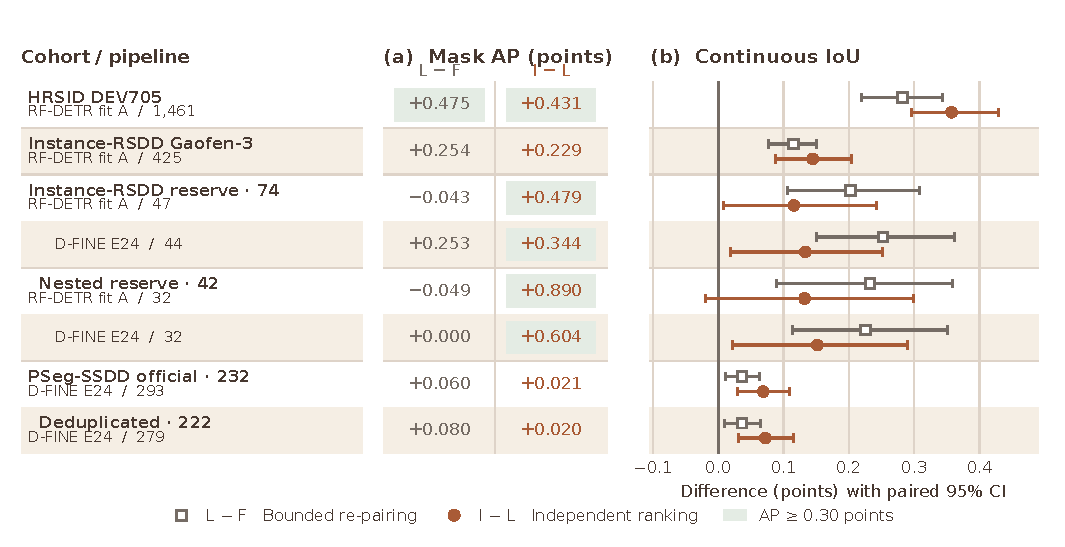
\includegraphics[width=\textwidth]{figures/journal_20261126/transfer_effects.pdf}
\caption{Matched-count contrasts \(L-F\) and \(I-L\). (a) Mask AP, with shading at or above 0.30 points. (b) Continuous IoU differences with paired 95\% group intervals. Counts are eligible fixed matches.}
\label{fig:transfer-effects}
\end{figure*}

\subsection{Frozen transfer to Instance-RSDD}
Instance-RSDD~\cite{rsdd} annotates ship outlines on RSDD-SAR imagery~\cite{rsddsar}. We use the released split of 2,810 training chips and 740 test chips. The dataset paper lists 2,840 and 715, respectively. The released test chips contain 872 outlines, and all 112 test parent scenes also occur in the published training split. The RF-DETR detectors and their scalar ROHs were fitted on HRSID before transfer. The prespecified Gaofen-3 subset contains 583 chips, 631 outlines and 76 acquisitions from a sensor absent from HRSID fitting. TerraSAR-X supplies the remaining 157 test chips.

At equal counts, independent selection improves AP with both Gaofen-3 detectors (Table~\ref{tab:primary-quant}). With fit A, the two scalar ROH fits gain 0.482--0.483 AP points and a mean of 0.259 continuous IoU points (\([0.194,0.322]\)) across 425 eligible matches in 68 acquisitions. With fit B, the three gains range from 0.240 to 0.378 AP points. The gains average 0.299 AP and 0.196 IoU points (\([0.136,0.253]\)) across its own 425 matches in 67 acquisitions. At the natural count with fit A, AP and AP75 increase by 0.517--0.587 and 1.230--1.438 points over the native masks, while AP90 drops by 0.094--0.107 points. Across all 740 chips, the mean natural-count AP gains are 0.539 and 0.435 points for fits A and B.

The fixed-count improvement also occurs on the 74-chip reserve, drawn from 13 additional parents in the published training split. With detector fit A and the first scalar ROH, independent selection gains 0.436 AP and 0.318 continuous IoU points (\([0.217,0.436]\)) across 47 eligible matches. Its nested 42-chip date-separated view contains 32 eligible matches and gives gains of 0.840 AP and 0.364 IoU points (\([0.250,0.478]\)). Fit B contributes 48 and 31 eligible matches in the full and nested views. Its means over three ROH fits give gains of 0.306 and 0.529 AP points and 0.267 and 0.326 IoU points, with respective IoU intervals \([0.161,0.374]\) and \([0.166,0.460]\). Both fits meet the 20-match and eight-parent coverage criteria in each view. Intervals resample sensor--date blocks, with equal weights for parent scenes. The nested view tests sensitivity to close acquisition dates within the reserve. Geographic independence remains unverified.

For independent selection over distance pairing, the one-pixel Boundary IoU intervals are positive for Gaofen-3 fit A and the 74-chip reserve, and span zero for Gaofen-3 fit B (Table~\ref{tab:native-boundary}). All three two-pixel intervals are positive. The native and reference masks retain eroded interiors at both widths. The reserve has 47 eligible matches across 12 parents. Its one-pixel interval is \([0.231,1.243]\) with sensor--date block resampling.

\begin{table}[t]
\centering
\caption{Fixed-match Boundary IoU contrasts (points). Paired 95\% intervals resample acquisitions on Gaofen-3 and parent scenes on the reserve.}
\label{tab:native-boundary}
\footnotesize
\setlength{\tabcolsep}{2.5pt}
\begin{tabular}{@{}lcc@{}}
\toprule
Cohort and comparison & One pixel & Two pixels\\
\midrule
Gaofen-3, fit A & \(+0.466\ [0.223,0.702]\) & \(+0.467\ [0.278,0.653]\)\\
Gaofen-3, fit B & \(+0.177\ [-0.025,0.376]\) & \(+0.255\ [0.107,0.404]\)\\
Reserve, paired & \(+0.701\ [0.180,1.233]\) & \(+0.617\ [0.236,1.001]\)\\
Reserve, PointRend & \(+0.829\ [-0.056,1.750]\) & \(+0.801\ [0.285,1.370]\)\\
\bottomrule
\end{tabular}
\end{table}

\subsection{Re-pairing within the distance cap and removing the cap}
\label{sec:pairing-effects}
Does a better choice of partners suffice, or does removing the distance cap yield a further gain? Figure~\ref{fig:transfer-effects} and Table~\ref{tab:bounded-results} report \(L-F\) for the first comparison and \(I-L\) for the second. Each row holds the detector, scalar ROH, support and per-side count \(k\) fixed. The prespecified criterion requires a gain of at least 0.30 mask AP points, a same-direction 95\% continuous-IoU interval and at least 20 changed eligible matches across eight groups. The 42-chip reserve view and 222-image PSeg view are nested within their respective cohorts.

\begin{table*}[!t]
\centering
\caption{Effects of bounded re-pairing ($L-F$) and of removing the distance cap ($I-L$) at matched signed counts, in points. Brackets give paired 95\% intervals for continuous IoU. Both detector pipelines use the same 74 reserve chips.}
\label{tab:bounded-results}
\footnotesize
\setlength{\tabcolsep}{4pt}
\renewcommand{\arraystretch}{1.12}
\begin{tabular}{@{}llrrrrl@{}}
\toprule
\multicolumn{2}{@{}l}{Evaluation view} & Eligible & \multicolumn{2}{c}{\(L-F\)} & \multicolumn{2}{c@{}}{\(I-L\)}\\
\cmidrule(lr){4-5}\cmidrule(l){6-7}
Cohort & Pipeline & matches & AP & Continuous IoU [95\% CI] & AP & Continuous IoU [95\% CI]\\
\midrule
HRSID DEV705 & RF-DETR fit A & 1,461 & \(+0.475\) & \(+0.282\ [0.219,0.344]\) & \(+0.431\) & \(+0.357\ [0.296,0.429]\)\\
Instance-RSDD Gaofen-3 & RF-DETR fit A & 425 & \(+0.254\) & \(+0.115\ [0.078,0.150]\) & \(+0.229\) & \(+0.145\ [0.087,0.204]\)\\
Instance-RSDD reserve 74 & RF-DETR fit A & 47 & \(-0.043\) & \(+0.203\ [0.107,0.308]\) & \(+0.479\) & \(+0.116\ [0.008,0.242]\)\\
 & D-FINE E24 & 44 & \(+0.253\) & \(+0.252\ [0.151,0.362]\) & \(+0.344\) & \(+0.133\ [0.018,0.251]\)\\
\quad Nested 42 & RF-DETR fit A & 32 & \(-0.049\) & \(+0.232\ [0.089,0.359]\) & \(+0.890\) & \(+0.132\ [-0.020,0.299]\)\\
 & D-FINE E24 & 32 & \(0.000\) & \(+0.225\ [0.114,0.351]\) & \(+0.604\) & \(+0.151\ [0.021,0.290]\)\\
PSeg-SSDD official & D-FINE E24 & 293 & \(+0.060\) & \(+0.037\ [0.011,0.063]\) & \(+0.021\) & \(+0.069\ [0.030,0.109]\)\\
\quad Deduplicated 222 & D-FINE E24 & 279 & \(+0.080\) & \(+0.037\ [0.009,0.064]\) & \(+0.020\) & \(+0.072\ [0.031,0.116]\)\\
\bottomrule
\end{tabular}
\end{table*}

Both increments meet the criterion on HRSID. On Gaofen-3, the IoU intervals are above zero, while the AP gains fall below the practical threshold. On the historical 74-chip reserve, \(I-L\) meets the criterion with both frozen pipelines. D-FINE changes 42 of 44 eligible matches across 11 sensor--date blocks. RF-DETR and D-FINE use separately trained detector and scalar ROH combinations and share the same target chips.

At one native pixel on the reserve, \(L-F\) gains 0.735 Boundary-IoU points with RF-DETR and 0.639 with D-FINE. The paired 95\% sensor--date-block intervals are \([0.298,1.217]\) and \([0.271,1.052]\), respectively. The corresponding \(I-L\) effects are \(-0.034\) points with RF-DETR (\([-0.380,0.287]\)) and \(+0.256\) with D-FINE (\([-0.176,0.697]\)). Resampling parent scenes for RF-DETR gives intervals of \([0.207,1.243]\) for \(L-F\) and \([-0.373,0.278]\) for \(I-L\). At two pixels, both detectors also have \(I-L\) intervals that span zero. The continuous-overlap gains after removing the cap therefore leave the narrow-contour improvement uncertain. With the adapted PointRend scores at the same cap and counts, \(I-L\) changes AP by \(+0.095\) points and continuous IoU by \(-0.037\) (\([-0.172,0.086]\)). The ROH-minus-PointRend interaction is \(+0.153\) IoU points (\([-0.008,0.339]\)).

On PSeg-SSDD, the \(I-L\) AP gain is small on both the full and deduplicated views. On all 232 images, the all-hull raster IoU effect is \(+0.040\) points under PSeg and \(-0.007\) under SPSD, each using its own native assignments. The paired SPSD-minus-PSeg difference is \(-0.047\) points (\([-0.088,-0.007]\)). The images are identical, while the reference contours and their original candidate assignments can differ.

We also restrict independent writes to candidates on which the selected endpoints cannot be paired within the cap and the minimum summed squared pair distance does not exceed that for either pairing comparator. On DEV705 this rule changes 36 candidates across 19 prefixes and just one of 1,461 eligible matches. It fails the coverage requirement and changes AP by \(-0.0014\) points relative to bounded re-pairing. On the 74-chip reserve, the SSDD-trained SRNet comparison gives \(+0.145\) AP and \(+0.159\) continuous IoU points (\([0.088,0.236]\)) for independent selection over distance pairing. The AP gain falls below the criterion.

\subsection{Frozen transfer to PSeg-SSDD}
On PSeg-SSDD, the same frozen D-FINE detections allow direct comparisons of placement rules under a new set of annotated contours. On DEV187 all five policies retain the same 18,700 candidates, including empty masks (Table~\ref{tab:ssdd}).


At identical counts on DEV187, independent selection gains 0.071 AP and 0.112 continuous IoU points over distance pairing (\([0.048,0.178]\)) on 209 fixed matches in 111 image groups. No match exceeds 0.90. The natural-count writer gains 0.336 AP points over native and 0.278 over distance pairing, below the respective 0.50- and 0.30-point margins. Deduplication preserves these directions. Acquisition independence remains unverified.

The HRSID-trained detector and ROH give a similar pattern on the historical official split. At the natural count, mask AP rises from 17.974 to 18.319 and AP75 from 13.015 to 14.705. Holding the count fixed yields an AP gain of 0.081 points over distance pairing. Ten official test images share decoded content with the historical PSeg training allocation. Excluding them leaves gains of 0.389 AP points for the natural-count comparison with native and 0.100 for independent selection over distance pairing at the same count.

Across 293 editable matches, independent selection adds 0.106 continuous IoU points over fixed pairing at the paired count, with an image-paired 95\% interval of \mbox{\([0.055,0.157]\)}. The natural-count writer gains 0.228 points over native (\([0.104,0.364]\)). All matches remain below 0.90. With oracle ranks, the natural-count masks could gain a further 1.097 IoU points. Allowing unequal signed counts at the same total adds 2.020 more points in the oracle comparison.

At the dynamic attraction budget~\cite{atkinson}, both writers make 73,770 exchanges on 11,054 candidates. Learned ranking scores 18.331 AP, compared with 18.357 for dynamic attraction. It improves AP75 by 0.279 points and loses 0.270 continuous IoU points (\([-0.440,-0.098]\)). Deduplication preserves these directions. Independent selection improves continuous overlap over distance pairing at the original paired count, while attraction gives the higher overlap at the dynamic count.

On historical DEV187, we also test the HRSID ROH on an RF-DETR E24 detector trained on PSeg. At the dynamic budget, learned and dynamic rankings score 69.958 and 69.113 AP, respectively. The continuous-IoU gain of 0.193 points fails the criterion, with a 119-group paired 95\% interval of \([-0.036,0.430]\). The native masks score 70.694 AP and lead the learned writer by 0.735 AP and 0.404 IoU points (\([0.245,0.564]\)). Independent selection at the fixed-pair count gains 0.279 AP and 0.097 IoU points over distance pairing (\([-0.035,0.232]\)).

The reference-guided comparison leaves room to improve endpoint rankings on this detector. On 281 matches, polygon-optimal ranks at the attraction count exceed native by 2.246 continuous IoU points and learned ranks by 2.651. Allowing fewer flips on the same support adds 0.032 points beyond that optimum. Allowing the mask area to change at the same total count adds 1.018 points. These ceilings apply to the evaluated support and reference polygons.

Refitting on PSeg leaves a gap to the native masks on DEV187. The refit uses 109 PSeg training images and 200 updates, with zero decoded-image overlap with DEV187. At the attraction count it scores 69.809 AP, which is 0.695 points above dynamic attraction, 0.150 below frozen transfer and 0.885 below native. Continuous IoU falls by 0.470 points from native (\([-0.621,-0.325]\)). The AP result retains its direction after deduplication, and the refit misses the replication criterion.

\begin{table}[t]
\centering
\caption{Frozen HRSID-to-PSeg-SSDD mask AP on DEV187. Dedup.\ uses float polygons on 182 unique decoded images.}
\label{tab:ssdd}
\footnotesize
\begin{tabular}{@{}lrrr@{}}
\toprule
Mask policy & Float & Integer & Float, dedup. \\
\midrule
Raw D-FINE E24 & 17.897 & 16.804 & 18.261 \\
ROH, fixed pairing & 17.956 & 16.877 & 18.329 \\
Independent, fixed-policy count & 18.028 & 17.173 & 18.393 \\
\midrule
Independent, natural count & 18.234 & 17.557 & 18.620 \\
Native ranks, natural-policy count & 17.942 & 16.757 & 18.308 \\
\bottomrule
\end{tabular}
\end{table}

\subsubsection{Sensitivity to the reference masks}
An unchanged prediction can receive different overlap scores when two releases trace the same ship differently. PSeg-SSDD and SPSD~\cite{slgsea} supply different reference masks for the same 232 byte-identical JPEGs. We evaluate the same 23,200 D-FINE candidates, ranks, masks and edit locations against both releases. PSeg uses rasterized polygons, while SPSD area and bounds follow the original raster instance IDs. A within-image one-to-one association yields 544 reference pairs with median raster IoU of 0.747 and median SPSD-to-PSeg area ratio of 0.822. At mask IoU 0.50 the native masks match 402 of 546 PSeg hulls and 403 of 547 SPSD hulls.

The reference changes the measured effect of an unchanged edit. At the paired count, independent selection improves AP by \(+0.081\) points over distance pairing on PSeg and changes it by \(-0.007\) on SPSD. At the natural count, its AP effect relative to native shifts from a gain of \(0.344\) points to a loss of \(0.491\). The all-hull raster IoU effect shifts from \(+0.119\) to \(-0.240\) points. The difference is \(-0.359\) points (\([-0.479,-0.247]\)), with identical decoded-image bootstrap draws and separate native match assignments for the two references. At the same attraction count, learned ranking loses \(0.086\) AP points to static attraction on PSeg and \(0.946\) on SPSD.

Most of the natural-count shift comes from edited cells that the two references label differently. Among 493 reference pairs with mutual IoU of at least 0.50, 358 share a native candidate. Natural-count editing changes 262 of these candidates in 137 images. For reference \(R\), the fixed-area IoU effect is \(a_R g_R\), where \(g_R\) is the signed intersection gain in Eq.~\eqref{eq:intersect-changes} and \(a_R\) is its IoU scale. The term \(\bar a(g_{\rm SPSD}-g_{\rm PSeg})\) isolates the contribution of cells with differing labels. At the original 232-image weights, this term accounts for \(-0.286\) points (\([-0.388,-0.193]\)) of the \(-0.359\)-point total shift. Changing the IoU scale on the same candidates adds \(-0.013\) points. Assignment, reference counts and unpaired hulls account for the remainder. The corresponding conflicting-label terms are \(-0.313\) points (\([-0.440,-0.193]\)) for learned ranking against static attraction and \(-0.037\) points (\([-0.081,+0.006]\)) for independent selection against distance pairing (Fig.~\ref{fig:reference-disagreement}). Among shared natural-count matches whose references agree at IoU 0.75 or higher, the term is \(-0.102\) points (\([-0.163,-0.046]\)) under the same original image weights. The comparison quantifies reference sensitivity among the released masks. The physical outline of an individual hull remains undetermined.

\begin{figure*}[!t]
\centering
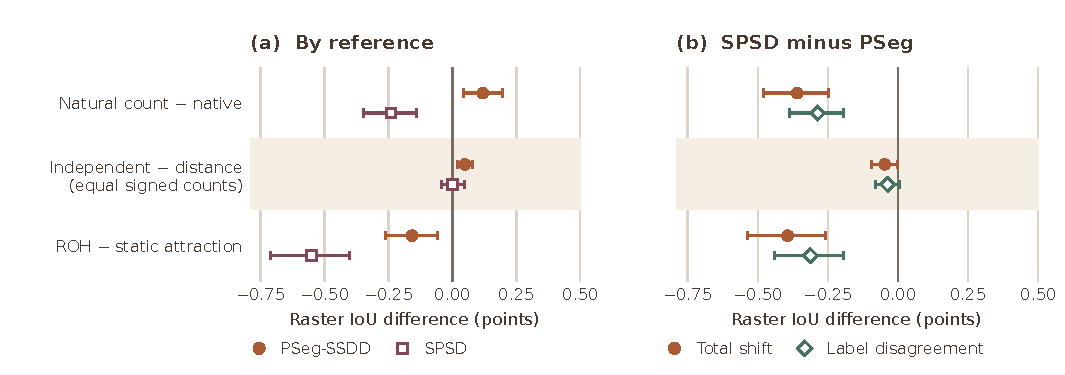
\includegraphics[width=0.98\textwidth]{figures/journal_20261126/reference_disagreement_effects.pdf}
\caption{Reference sensitivity on the same 232 SSDD images and writer outputs. (a) All-hull raster-IoU effects using each reference's native assignments. (b) SPSD-minus-PSeg effect and its label-disagreement component. Intervals use paired 95\% decoded-image-group resampling; the two references are not separate acquisition cohorts.}
\label{fig:reference-disagreement}
\end{figure*}


\subsubsection{Variable signed allocation at the same total count}
\label{sec:variable-sign-results}
The two SSDD releases let us ask whether a change in mask area helps under both annotations of the same images. Each reference retains its own native assignments. The decomposition for the first dual-reference head fit uses paired resampling of decoded-image groups.
At 115,384 total flips across 18,300 candidates, the variable allocation improves mask AP and raster IoU under both SSDD references. Both rules use the same two predicted foreground probabilities at each endpoint and the same predicted-IoU objective. Fitting candidates come from 732 images in the published training split, 447 of which contribute to the common positive-budget set. The 183 historically used development images belong to decoded-image groups excluded from fitting. The equal-allocation control makes 57,692 additions and 57,692 removals. For the initial dual-reference ROH fit, variable allocation makes 67,777 additions and 47,607 removals. Its gain is 2.461 mask AP and 0.993 fixed-match raster IoU points on PSeg (\([0.747,1.244]\)), and 1.782 AP and 0.580 IoU points on SPSD (\([0.298,0.877]\)). The fixed-area robust and mean BCE writers also score lower on the two references. 

With the split range held fixed, the mean-IoU objective gains 0.498 AP and 0.312 IoU over the maximin objective on PSeg, while losing 0.044 AP and 0.073 IoU on SPSD. The mean objective thus trades a gain on PSeg against a loss on SPSD.

To separate the change in intersection from the change in predicted area, let \(P_0,P_1\) and \(I_0,I_1\) denote the fixed and variable writers' areas and intersections against one reference. Define \(U_j=P_j+T-I_j\), \(\bar P=(P_0+P_1)/2\), and \(\bar I=(I_0+I_1)/2\). The exact IoU difference is
\begin{equation}
 \Delta\mathrm{IoU} =
 \frac{(\bar P+T)(I_1-I_0)-\bar I(P_1-P_0)}{U_0 U_1}.
 \label{eq:area-overlap-parts}
\end{equation}
The additional intersection accounts for 2.243 IoU points on PSeg and 2.041 on SPSD. The area terms offset these gains by \(-1.250\) and \(-1.461\) points (Fig.~\ref{fig:dual-budget-effect}). The mean absolute area errors across groups fall by 4.705 and 1.520 cells, respectively. Among 206 common positive-budget hulls, 182 gain reference intersection under both labels and five lose under at least one. The larger masks thus recover annotated hull area on these images. The reference-area proxy in Eq.~\eqref{eq:dual-area-proxy} relies on the native foreground outside the sampled sites, where both references locate about 78\% of the static-mask error.


The variable split improves overlap in both additional fits of the dual-reference ROH (Table~\ref{tab:dual-sign-seeds}). For each of the three fits we compare its own equal- and variable-allocation outputs on the same development images. Mean gains are 2.299 AP and 0.971 fixed IoU points on PSeg, and 1.751 AP and 0.573 IoU points on SPSD. The IoU intervals are \([0.740,1.207]\) and \([0.319,0.840]\), respectively. The intervals resample evaluation groups after averaging the three fits within each group.

Replacing the ratio approximation with the exact objective in Eq.~\eqref{eq:exact-iou-signed} preserves the gain on the initial dual-reference ROH fit. At the same total count, it changes the variable and fixed choices on 136 and 11 of 8,785 positive-budget candidates, respectively. All 206 common positive-budget matches retain the variable mask. Both references give identical AP and fixed-match IoU for each approximation and exact-objective pair. This checks the reciprocal-moment approximation under independent endpoint Bernoulli labels and deterministic native labels outside the writable support. Modeling the spatial dependence studied by RankSEG-DEP~\cite{rankdep} requires a different joint distribution. At fixed signed counts, the expected intersection in Eq.~\eqref{eq:independent-estimated-gain} is linear in the occupancy marginals.

A joint model improves predictions for adjacent endpoint pairs with little change in the masks. It holds the occupancy marginals fixed while modeling disjoint four-neighbor pairs, with independence and sign-preserving rewiring as controls. On held FIT groups, local dependence reduces the four-state Brier loss by 0.058 and 0.089 under the two references relative to independence on the same pairs. Freezing the coefficients and rescoring the same signed menus changes one of 206 common positive-budget masks on development. Mask AP is identical under both references. Raster IoU changes by zero and \(+0.00175\) points, with the latter interval spanning zero.

\begin{table}[t]
\centering
\caption{Variable minus equal allocation with the same total number of flips, in points. Each of the three dual-reference ROH fits is evaluated on the same SSDD images.}
\label{tab:dual-sign-seeds}
\footnotesize
\begin{tabular}{@{}lrrrr@{}}
\toprule
 & \multicolumn{2}{c}{PSeg-SSDD} & \multicolumn{2}{c}{SPSD}\\
\cmidrule(lr){2-3}\cmidrule(lr){4-5}
ROH fit & AP & IoU & AP & IoU\\
\midrule
1 & 2.461 & 0.993 & 1.782 & 0.580\\
2 & 2.465 & 1.037 & 1.615 & 0.584\\
3 & 1.971 & 0.882 & 1.856 & 0.555\\
\midrule
Mean & 2.299 & 0.971 & 1.751 & 0.573\\
\bottomrule
\end{tabular}
\end{table}

With the dual-reference ROH and policy frozen on the 232 SAR-SSP validation chips, the variable split changes 48 original matches in 20 parent scenes. The mask AP and fixed-match IoU point estimates are \(-0.139\) and \(-0.212\) points (\([-0.547,0.104]\) for IoU). It reduces missed area by 0.653 points of reference area (\([-1.079,-0.328]\)) and adds 1.378 points of excess foreground (\([0.750,2.067]\)). Against the released raster masks of this previously evaluated cohort, recovery of missed area comes with excess foreground. The paired transfer criterion is unmet. Substituting exact expected IoU for the ratio changes the variable actions on 142 of 10,393 candidates. AP and fixed IoU still agree for each allocation arm.

A reference-assisted comparison shows more potential gain in the split than in the ranking within that split. We replay the original menus for the 50 native matches with positive edit counts and retain the 139-hull denominator. Choosing the best action at the predicted split using the reference mask gains 0.180 mother-scene-weighted IoU points. Searching all splits after this replacement adds another 1.147 points. A separate substitution preserves the predicted winner for each split and uses the reference to choose only the split. It recovers 0.958 points. Replacing the predicted reference area and static intersection by exact values while preserving predicted intersection changes yields a 0.005-point effect (\([-0.096,0.115]\)). These reference-dependent checks describe available actions on this cohort.

The extra false foreground almost always extends an existing component. Of 393 false foreground cells present only under variable allocation, 392 belong to the largest component containing a retained fixed-mask cell, under either four- or eight-neighbor connectivity. Net excess consists of 162 cells added outside the native mask and 175 native cells retained by variable allocation. Their scene-weighted contributions are 0.667 and 0.711 points of reference area. Isolated additions account for one gained false foreground cell on the original matches.

At the differing edit sites, the two source-fitted outputs overestimate the intersection gain on SAR-SSP by 0.896 and 0.628 points of reference area. Against their respective SSDD references, the analogous overestimates are 0.089 and 0.231 points. Negative target area-coefficient terms partly offset the intersection error in both outputs. The calculation conditions on the selected edits. Both outputs use the same SAR-SSP reference, and each source or target view retains its own grouping.

\begin{figure*}[!t]
\centering
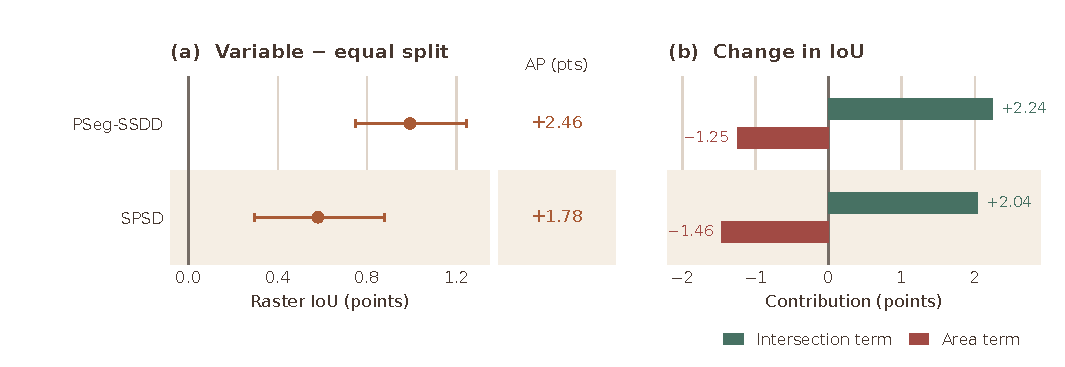
\includegraphics[width=0.98\textwidth]{figures/journal_20261126/dual_reference_budget_effect.pdf}
\caption{Changing the allocation of 115,384 flips on the same 183 SSDD development images. (a) Variable-minus-equal differences in raster IoU and mask AP for the first dual-reference ROH fit. IoU intervals use paired 95\% decoded-image-group resampling. PSeg and SPSD annotate the same images. (b) Exact contributions of intersection and mask area to the IoU change. Table~\ref{tab:dual-sign-seeds} gives the mean over three fits.}
\label{fig:dual-budget-effect}
\end{figure*}

\subsection{Comparisons with strong ranking and full-mask alternatives}
Spatial attraction provides a geometric alternative to an occupancy score for ranking the same cells. At the dynamic-attraction count on the 74-chip reserve, ROH ranking improves continuous overlap over both attraction rules. The gain over dynamic attraction is 0.468 AP and 0.431 IoU points (\([0.213,0.662]\)). Over static attraction it is 0.203 AP and 0.301 IoU points (\([0.088,0.534]\)), although static leads by 0.173 AP75 points. Both comparisons change 47 eligible masks in 11 sensor--date blocks. The date-separated AP gains are 0.978 and 0.478 points. Neither individual sensor group meets the minimum coverage required for this comparison.


The stricter AP90 contrast depends on the overlap convention. On Gaofen-3 fit B, learned minus dynamic changes from \(-0.149\) points under raster overlap to \(+0.004\) under polygon--cell overlap, with a paired 95\% interval for the shift of \([-0.195,0.579]\). On fit A, it falls from \(+0.279\) to \(+0.053\). Both conventions share the same 631 outlines and prediction identities and order. The mean AP advantage across the ten thresholds is positive for both fits. The AP90 comparison therefore depends on the available matches and the overlap convention.

Five-pass Phoenix XL1~\cite{phoenix} provides a learned ranking comparison on the same endpoints and counts. On the 74 chips, disabling its 1\% gate for this comparison gives Phoenix 58.976 AP and a 0.308-point AP gain over ROH ranking. Continuous IoU differs by 0.135 points (\([-0.026,0.277]\)). Replacing only the Phoenix additions with ROH choices changes mean AP by \(-0.012\) points. Replacing only the deletions changes it by \(-0.225\). Both intersection intervals span zero. With image-only shifts of \(\pm1\) column, the mean signed centroid response is 0.117 pixels for Phoenix and 0.070 for ROH ranking (paired difference 0.047, \([0.028,0.064]\), 47 hulls). This perturbation measures alignment sensitivity on fixed proposals. It leaves the source of the ranking difference on correctly aligned images unresolved.

The PointRend comparison holds the endpoints and the counts from the first scalar ROH fit fixed. Both heads use row-major ordering for ties and operate on capped or complete two-layer box support. The binary PointRend head uses HRSID FIT109 RF-DETR features, 200 updates at 196 targets per update, 3,136 evaluations per RoI and zero padding. The two predictors use different features and supervision.

\begin{table}[t]
\centering
\caption{Matched-support ranking on Gaofen-3. Both rankers make 268,347 exchanges. Continuous IoU weights acquisitions equally over 425 fixed matches.}
\label{tab:rsdd-pointrend}
\setlength{\tabcolsep}{4pt}
\begin{tabular}{lrrrr}
\toprule
Policy & AP & AP75 & AP90 & IoU\\
\midrule
Native RF-DETR & 61.033 & 71.822 & 3.256 & 79.652\\
Coarse RoI paste & 53.880 & 56.474 & 1.486 & 75.108\\
PointRend RoI paste & 61.831 & 74.396 & 3.227 & 79.939\\
\midrule
PointRend ranks, capped & 61.309 & 72.646 & 3.017 & 79.647\\
ROH ranks, capped & 61.620 & 73.259 & 3.162 & 79.897\\
PointRend ranks, complete & 61.241 & 72.525 & 3.015 & 79.648\\
ROH ranks, complete & 61.631 & 73.280 & 3.041 & 79.871\\
\bottomrule
\end{tabular}
\end{table}

At identical counts, ROH ranks outperform PointRend ranks on both supports (Table~\ref{tab:rsdd-pointrend}). Gains are 0.312 AP and 0.250 continuous IoU points on capped support (\([0.163,0.338]\)) and 0.390 AP and 0.223 IoU points on complete support (\([0.123,0.330]\)). Removing the cap changes the ranking gaps by \(+0.078\) AP and \(-0.027\) IoU points (\([-0.086,0.028]\)).

The full PointRend paste gains 0.200 AP points over ROH ranking on complete support, with lower AR100 (72.361 versus 74.105). Of its differences from capped PointRend ranks, 90.6\% lie outside capped support. Capping the paste gives 61.782 AP and 73.566 AR100 at unequal counts. On complete support, 25.2\% of PointRend deletions and 3.4\% of ROH deletions lie outside the RoI. Full pasting changes both the set of writable cells and the output area. Its AP and recall address a broader comparison than ranking identical endpoints.

Restricting all 268,302 exchanges to the clipped RoI retains the ROH advantage. With zero padding, the gains are 0.379 AP and 0.224 IoU points (\([0.125,0.329]\)). Border replication gives 0.345 AP and 0.223 IoU points (\([0.124,0.327]\)). The padding change accounts for 0.034 AP and 0.001 IoU points (\([-0.006,0.008]\)).

On the 74-chip reserve, ROH ranking gains 0.477 AP and 0.395 IoU points over capped PointRend at 31,391 exchanges (\([0.204,0.620]\) for IoU). On the date-separated view the corresponding gains are 1.061 AP and 0.490 IoU points (\([0.225,0.751]\)). On the full reserve the one-pixel Boundary IoU interval includes zero and the two-pixel interval lies above zero (Table~\ref{tab:native-boundary}). The nested view gives \(+1.397\) one-pixel points \([0.245,2.420]\) over 32 matches in eight parents.

ROH ranking also improves PointRend when the original paste supplies the per-mask signed counts and the mask outside capped support. AP improves in all three ROH fits. The mean increases from 57.534 to 58.196 on the 74 chips and from 61.831 to 61.975 on Gaofen-3. Continuous IoU gains 0.251 and 0.195 points, with intervals of \([0.051,0.449]\) and \([0.109,0.281]\). The writers choose different sites on 44 of 47 matches in 12 parents and 424 of 425 in 68 acquisitions. We average the head effects per match, then draw 4,096 paired sensor--date resamples with equal parent weights or acquisition resamples with equal acquisition weights. In the date-separated view the gains are 0.781 AP and 0.284 IoU points (\([-0.007,0.528]\)). The standalone ROH writer on capped support scores 58.827 AP on the full 74 chips.

The original Phoenix XL1 binary update can modify the whole mask. On the same reserve, we apply it with five refinement iterations and the published COCO and LVIS area gates. The COCO rule admits the 172 candidates whose foreground exceeds 1\% of the image and excludes the 32--1023-pixel range used by NORA. The LVIS rule refines all 6,079 nonempty native masks. Both preserve the scores and all 7,346 candidate identities. They give identical outputs for the 172 candidates refined by both. Thresholding the retained Phoenix scores at 0.50 independently reproduces the full-mask decisions on all 259,242 recorded endpoints in 4,107 matched-budget candidates.

\begin{table}[t]
\centering
\caption{Phoenix writers on the 74-chip Instance-RSDD reserve. Hull counts use COCO rematching at IoU 0.50 among 81 reference hulls.}
\label{tab:phoenix-whole}
\footnotesize
\begin{tabular}{@{}lrrr@{}}
\toprule
Mask policy & AP & AR100 & Hulls\\
\midrule
Native RF-DETR & 58.277 & 73.457 & 81\\
ROH, matched count & 58.668 & 73.992 & 81\\
Phoenix, matched count & 58.976 & 73.951 & 81\\
Phoenix whole, COCO gate & 58.161 & 73.210 & 81\\
Phoenix whole, LVIS gate & 41.198 & 57.654 & 73\\
\bottomrule
\end{tabular}
\end{table}

The LVIS-policy write loses 17.779 AP and 9.825 continuous IoU points relative to matched Phoenix (Table~\ref{tab:phoenix-whole}). The paired 95\% IoU interval is \([-14.014,-6.440]\) over 47 original eligible matches and 11 sensor--date blocks. False-positive area increases by 33.726 points of reference area (\([19.461,50.351]\)). Missed area changes by \(-2.905\) points (\([-5.907,0.286]\)). At IoU 0.50, 65 of 81 original hull associations survive and rematching reaches 73 hulls. On the date-separated view AP falls by 19.137 points and IoU by 11.327. Both sensor views give the same sign, with fewer than eight contributing date blocks per sensor. These effects apply to this historical detector stream and reflect joint changes in write support, area and eligibility.

With its original 512-pixel mask gate and six denoising steps, the published COCO SegRefiner-LR writer modifies 3,074 of 7,346 native candidates on the reserve. Its mask AP is 56.574, compared with 58.277 for native and 58.827 for independent ROH ranking. Continuous IoU falls by 3.809 points from native in the full fixed-match set (\([-6.078,-1.388]\)) and by 4.207 among the 39 matched hulls it edits (\([-6.481,-1.542]\)). Across the full fixed-match set, excess foreground falls by 2.824 points of reference area while missed hull area increases by 6.266. The direction persists in the 42-chip date-separated view.

The stock deletions reduce continuous IoU on the 39 gate-exposed matches by 4.092 points before additions and 4.087 after additions, with both paired intervals below zero. They remove 8.843 points of true hull area, while additions recover 1.675. Holding the additions and deletion count fixed, moving the deletions toward the native boundary gains 0.543 AP points over the stock writer. The geometry gain of 0.574 points has an interval of \([-0.076,1.416]\). Relative to an equally large proximity-only relocation, the gains are 1.291 AP and 0.838 IoU points (\([0.272,1.558]\)). The 42-chip view fails the joint relocation criterion.


\begin{table}[t]
\centering
\caption{Stock deletion effects on fixed-match continuous IoU (points). Brackets give paired 95\% intervals.}
\label{tab:stock-deletions}
\footnotesize
\setlength{\tabcolsep}{3pt}
\begin{tabular}{@{}lrr@{}}
\toprule
Gate-exposed subset & Deletes vs.\ native & Stock vs.\ adds \\
\midrule
Instance-RSDD (39) & \(-4.09[-7.18,-0.96]\) & \(-4.09[-7.15,-0.99]\) \\
PSeg-SSDD (67) & \(-4.03[-5.22,-2.75]\) & \(-3.98[-5.16,-2.71]\) \\
\bottomrule
\end{tabular}
\end{table}

On PSeg-SSDD, the same stock writer modifies 5,067 of 23,200 native D-FINE candidates. It scores 17.136 AP. The native, local ROH and static ranker scores are 17.974, 18.319 and 18.417. Across all 293 eligible original matches, the effect is \(-0.386\) continuous IoU points versus native (\([-0.950,0.153]\)) and \(-0.614\) versus local ROH (\([-1.190,-0.047]\)). The decisions persist in the 222-image view after excluding ten exact overlaps.

Deletions reduce overlap in both addition contexts on the 67 gate-exposed PSeg matches in 57 decoded-image groups (Table~\ref{tab:stock-deletions}). They remove 6.937 points of true hull area, while additions recover 3.174. Additions alone improve continuous IoU by 2.405 points (\([1.635,3.192]\)). With counts fixed, moving deletions toward the periphery changes AP by \(-0.141\) points and exposed IoU by \(-0.503\) relative to stock (\([-1.092,-0.030]\)). Over proximity-only relocation, the gains are 0.042 AP and 0.134 IoU points (\([-0.109,0.371]\)). Neither view meets the joint evaluation criterion.

\subsection{Frozen transfer to Sentinel-1 acquisitions}
Few native masks reach the matched-overlap threshold on the first UEIKAP cohort~\cite{ueikap}. The 108 chips contain 139 hulls from 18 acquisitions, and the protocol requires 20 positive-budget IoU-0.50 matches across eight acquisitions. D-FINE matches two hulls, both at zero budget. Eight ideal swaps could cover four hulls. RF-DETR has 17 positive-budget matches in four groups. Independent selection improves on fixed pairing by 0.515 IoU points within the represented groups. With unmatched hulls assigned zero change, the 18-group effect is 0.03014 points (paired 95\% interval \([0.00028,0.08025]\)). All 17 positive-budget matches remain below 0.75.

The boxes provide substantially higher coverage than their attached masks. RF-DETR has a box at IoU 0.50 or above for 100 hulls. For 90 of them, the mask associated with the highest-overlap box occupies less than half the reference area. The median area ratio is 0.301. With candidate reuse allowed in the per-hull ceilings, eight ideal swaps cover 18 hulls at IoU 0.50, and within-box reconstruction covers 129. Score-ordered box matching selects 99 masks below 0.50, including 90 positive budgets from 15 acquisitions. Equal-count independent selection gains 0.0043 IoU points across 18 acquisitions (\([-0.0008,0.0101]\)). None reaches 0.50. Box and mask matching choose different candidates for 16 of 17 shared hulls. The coverage and area results bound what small, area-preserving edits can achieve in this view.

The second UEIKAP cohort includes enough positive-budget matches to compare the rules across acquisitions. On 342 chips from 13 additional Danish acquisitions, RF-DETR matches 121 of 528 released hulls, with positive budgets on 120 matches in ten groups. At equal counts, independent selection gains 0.02954 continuous IoU points over distance pairing with unmatched hulls set to zero (group-equal 95\% interval \([0.00790,0.05198]\)). The matched-only gain is 0.12306 points (\([0.02106,0.21932]\)). At the dynamic-attraction count, learned ranking loses 0.05322 IoU points to attraction (\([-0.09777,-0.01562]\)). The natural-count gain over native is 0.00623 points (\([-0.02481,0.03017]\)). One fixed match reaches continuous IoU 0.75 under all local policies.

Full PointRend pasting further reduces coverage on these previously evaluated chips. The frozen FIT109 PointRend head refines native masks with area \([32,1024)\) pixels. At raster IoU 0.50, the native masks cover 121 case-focused hulls, the \(7{\times}7\) coarse pastes cover 111 and the \(224{\times}224\) PointRend pastes cover 30. PointRend recovers no new hulls relative to either comparison. Across all 528 hulls, fixed box associations show more missed hull area and continuous IoU losses of 4.1375 points from native and 3.4553 from the coarse paste.

\subsection{Frozen transfer to SAR-SSP}
\label{sec:sar-ssp}
To test the placement rules against released raster masks, the SAR-SSP comparison uses the COCO-initialized RF-DETR fit A and the first frozen HRSID ROH fit on all 232 validation chips. The release includes 139 ship instances from 31 Gaofen-3 parent scenes in AIR-SARShip-1.0~\cite{slgsea,airsarship}. All 31 parents occur in both SAR-SSP splits. Neither allocation was used to fit or select the detector or ROH. Sensor or acquisition date distinguishes this cohort from the 74-chip Instance-RSDD reserve. Same-acquisition overlap remains unresolved for 11 images in the separate Instance-RSDD test set.

COCO mask AP includes all 22,741 candidates and all chips. We use the released instance IDs on the 500-pixel grid, including 48 hull masks that touch a tile edge. For geometry, we freeze the native IoU-0.50 assignments of 92 matched hulls and assign zero change to the other 47. Each of the 23 ship-bearing parent scenes has equal weight and is resampled as a unit for the paired intervals.

\begin{table}[t]
\centering
\caption{Frozen RF-DETR on SAR-SSP (points). The paired and independent policies share one edit count. The attraction policies share a separate count.}
\label{tab:sar-ssp}
\footnotesize
\renewcommand{\arraystretch}{0.91}
\begin{tabular}{@{}lrrr@{}}
\toprule
Mask policy & AP & AP75 & AR100 \\
\midrule
Native & 21.392 & 19.781 & 34.676 \\
Distance paired & 21.390 & 19.781 & 34.604 \\
Independent, paired count & 21.386 & 19.254 & 34.820 \\
\midrule
Dynamic attraction & 21.485 & 19.577 & 34.892 \\
Static, attraction count & 21.508 & 20.328 & 35.108 \\
Learned, attraction count & 21.504 & 19.254 & 34.748 \\
\bottomrule
\end{tabular}
\end{table}

Independent selection has little effect on SAR-SSP at the RF-DETR paired count (Table~\ref{tab:sar-ssp}). The two writers share 57,565 exchanges and produce different masks on 52 matches from 19 scenes. Mask AP changes by \(-0.005\) points and scene-balanced raster IoU by \(+0.101\) points (\([-0.066,0.335]\)). Excluding edge-touching hulls gives \(+0.180\) IoU points (\([-0.012,0.442]\)). The AP change is below the prespecified 0.30-point threshold and both IoU intervals span zero. At the attraction count, learned ranking changes AP by \(+0.019\) points relative to dynamic attraction and \(-0.004\) relative to static attraction. Corresponding IoU effects are \(-0.044\) (\([-0.419,0.475]\)) and \(-0.228\) points (\([-0.608,0.204]\)). The larger effects on the earlier Gaofen-3 polygons do not recur on these raster masks.

The D-FINE E24 pipeline gives similarly small effects on the same 232 chips. With its frozen HRSID ROH, each policy makes 39,546 exchanges. Independent selection changes 47 of 88 native matches in 19 scenes. Mask AP is 13.344 for both native and distance pairing and 13.420 for independent selection. The scene-balanced IoU gain over distance pairing is \(+0.022\) points (\([-0.193,0.238]\)). At the attraction count, learned ranking loses 0.114 AP points to the dynamic rule and 0.059 to the static rule, with both overlap intervals spanning zero. Only four of the 51 unmatched hulls have a retained D-FINE box at IoU 0.50 or above. Both pipelines offer limited evidence for a benefit from changing endpoint ranks on this cohort.

A reference-assisted assignment quantifies how many RF-DETR misses the D-FINE candidates could recover. We keep the 92 RF-DETR native matches and assign D-FINE candidates one-to-one to remaining hulls at mask IoU 0.50. The reference masks allow 10 additional matches across three scenes, eight of them from one parent. The upper bound falls short of the prespecified five-scene criterion. Even with both candidate pools, no mask reaches IoU 0.50 for 37 of 139 hulls.

\onecolumn
\begingroup
\renewenvironment{figure*}[1][]{\par\noindent\begin{minipage}{\linewidth}\FigureContext}{\end{minipage}\par}
\section{Matched qualitative examples}
\par\noindent\hfil\begin{minipage}{.85\linewidth}
\label{sec:qualitative}
For each case, we follow one detection against its original reference hull. Positive and negative examples near their respective median changes show where recovered intersection outweighs lost intersection and where it falls short. At equal signed counts the choice of sites accounts for the difference. When the split varies, added foreground can cover both previously missed hull and nearby background.
\end{minipage}\hfil\par
\par\noindent\hfil\begin{minipage}{.85\linewidth}
\subsection{Independent ranking under matched signed counts}

Does removing the distance cap place more of a mask on the annotated hull? Figure~\ref{fig:rsdd-common-cap-cases} compares the native mask and the three edited masks for two retained D-FINE detections on the historical Instance-RSDD reserve. Across the 44 eligible fixed matches, independent selection improves continuous IoU for 25 hulls relative to bounded re-pairing, lowers it for 11, and ties for eight. Independent selection gains 0.18 IoU points at four swaps in the first case and loses 0.15 points at eight swaps in the second. All three edited masks in a row add and remove the same numbers of cells. At this constant mask area, a rise or fall in IoU reflects a corresponding change in the intersection with the ground-truth hull.
\end{minipage}\hfil\par
\begin{figure*}[!t]
\centering
\includegraphics[width=0.88\linewidth]{\CaseAsset{rsdd74_common_cap_cases.pdf}{rsdd74_common_cap_cases.pdf}}
\caption{Gain and loss cases near the respective median $I-L$ changes on the 74-chip Instance-RSDD reserve (D-FINE). Each writer adds and removes four cells in (a) and eight in (b). \CaseCaption{The $8\times8$ display grid averages mask coverage. Its last panel pools the signed foreground difference $I-L$.}{All methods share the SAR crop, scale and GT polygon outline within each case. The last panel shows the signed foreground difference $I-L$.} Case selection and IoU use native polygon--cell geometry.}
\label{fig:rsdd-common-cap-cases}
\end{figure*}

\smallskip\noindent\begin{minipage}[c]{.39\linewidth}
\subsection{Sources of intersection changes on HRSID DEV705}

The DEV705 cases separate the area recovered by additions from the area forfeited by removals. For the ROH fit in Fig.~\ref{fig:dev-cases}, changing from fixed pairing to independent selection improves 1,012 of the 1,461 fixed matches (69.3\%) and degrades 252 (17.2\%). The remaining 197 (13.5\%) differ by at most \(10^{-12}\) in continuous IoU. With the same number of edits in Fig.~\ref{fig:dev-cases}(a), the independent additions recover one more reference pixel-equivalent and the removals spare a further 1.5. IoU rises by 0.732 points. Neither policy's additions recover reference area in (b). The independent rule removes one additional pixel-equivalent of the hull and loses 0.316 IoU points. In this case, maximizing the estimated gain removes more of the reference hull.

\end{minipage}\hfill\begin{minipage}[c]{.57\linewidth}
\begin{figure*}[!t]
\centering
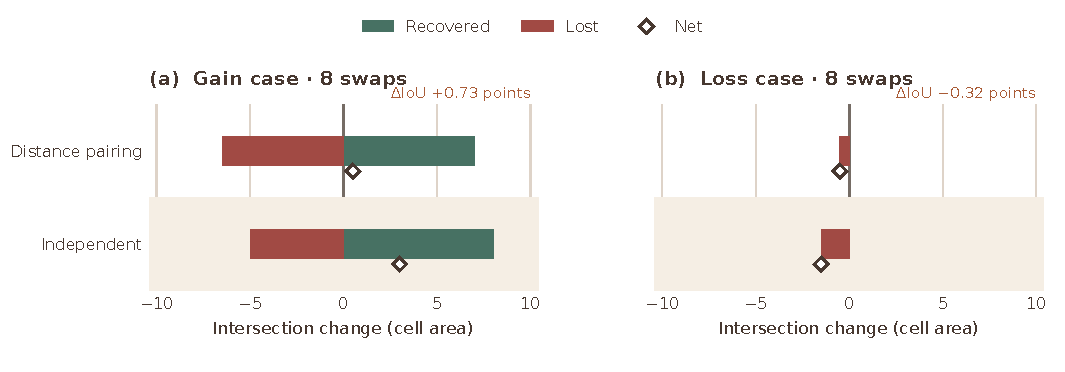
\includegraphics[width=1.0\linewidth]{figures/journal_20261126/dev705_overlap_cases.pdf}
\caption{Intersection area recovered by additions, lost to removals and gained overall relative to the native mask. The two RF-DETR DEV705 cases are near the median gain and median loss for independent versus distance-paired selection. Each rule adds and removes eight cells per case.}
\label{fig:dev-cases}
\end{figure*}

\end{minipage}\par
\clearpage
\par\noindent\hfil\begin{minipage}{.85\linewidth}
\subsection{Learned ranking and dynamic attraction on Gaofen-3}

ROH and dynamic attraction can place identical edit budgets on different parts of the contour. At the dynamic-attraction count, ROH ranking improves 268 of the 425 eligible matches from RF-DETR fit B (63.1\%), worsens 154 (36.2\%), and ties three. Figure~\ref{fig:gf3-qual} shows two gains and two losses, with eight swaps in each case. In the first two rows, the learned edits increase the reference intersection by 2.93 and 3.71 native pixel areas relative to dynamic attraction. The corresponding IoUs rise from 78.13 to 78.83 and from 71.86 to 72.56. In the other rows, the same number of edits reduces the intersection by 1.30 and 3.00 pixel areas. IoU falls from 87.09 to 86.52 and from 68.14 to 67.58.
\end{minipage}\hfil\par
\begin{figure*}[!t]
\centering
\includegraphics[width=0.97\linewidth]{\CaseAsset{gf3_matched_cases_binned.pdf}{gf3_cases_exact.pdf}}
\caption{ROH ranking and dynamic attraction with frozen RF-DETR fit B on Gaofen-3. Among 425 eligible matches, two cases are shown near the median gain and two near the median loss. Each rule adds and removes eight cells per case. \CaseCaption{An $8\times8$ display grid pools mask coverage and signed intersection differences. Coverage is shown in quarter-occupancy levels. The dashed GT contour marks 50\% coverage.}{Methods within each case share the SAR crop, scale and GT polygon outline.} Reported IoU and intersection areas use native geometry.}
\label{fig:gf3-qual}
\end{figure*}

\clearpage
\par\noindent\hfil\begin{minipage}{.85\linewidth}
\subsection{Whole-grid edit limits on PSeg-SSDD}

For a fixed whole-grid Phoenix response, limiting the number of flips improves 209 of 293 original eligible PSeg matches, worsens 76, and ties eight. In Fig.~\ref{fig:pseg-budget-cases}(A), the threshold mask recedes along the sides of the hull. Reducing the budget from 38 flips to 16 preserves \(17.87\) additional native pixel areas of the reference and raises IoU from 56.40 to 62.26. Native IoU is 66.88. In (B), thresholding recovers part of a narrow upper tip and raises IoU from 56.04 to 58.75. The fixed-count mask uses 16 flips. Its false-positive fraction falls from 1.26\% to 0.22\%, but it forfeits \(7.96\) native pixel areas of intersection and reaches 56.64 IoU. The constrained write spares correct side pixels in (A) and forgoes useful tip additions in (B).
\end{minipage}\hfil\par
\begin{figure*}[!t]
\centering
\includegraphics[width=0.98\linewidth]{\CaseAsset{pseg_budget_cases_binned.pdf}{pseg_budget_cases_exact.pdf}}
\caption{Fixed-count and thresholded Phoenix masks near the median gain and median loss on PSeg-SSDD. The count rule uses 16 flips in each case. Thresholding uses 38 in (a) and 75 in (b). \CaseCaption{Each bin of the $8\times8$ grid pools $5\times5$ native cells in (a) and $7\times7$ in (b). Coverage uses quarter-occupancy levels. The last panel pools the threshold-minus-count difference in FP+FN area.}{Methods share the SAR crop, scale and GT polygon within each case. The detail panel enlarges the marked boundary window.} IoU, FP and FN use native geometry. Error areas are expressed as percentages of GT hull area.}
\label{fig:pseg-budget-cases}
\end{figure*}

\clearpage
\par\noindent\hfil\begin{minipage}{.85\linewidth}
\subsection{Whole-crop refinement with SegRefiner}

Where the full-crop mask contracts determines whether it removes background or part of the hull. Of the 39 eligible original matches refined by SegRefiner-LR, 14 gain continuous IoU and 25 lose it. Figure~\ref{fig:segrefiner-cases} shows the cases closest to the median of each group. In (a), SegRefiner-LR trims an extension beyond the lower end of the ground-truth outline and raises IoU from 58.68 to 60.96. In (b), the refined mask loses intersection at both ends and along the narrow side, lowering IoU from 71.93 to 67.43. The local ROH masks score 58.89 and 71.95 on the same references.
\end{minipage}\hfil\par
\begin{figure*}[!t]
\centering
\includegraphics[width=0.97\linewidth]{\CaseAsset{rsdd74_segrefiner_cases_binned.pdf}{rsdd74_segrefiner_cases_SAR_PRIVATE.pdf}}
\caption{Gain and loss cases for SegRefiner-LR among 39 eligible Instance-RSDD matches. Native, local ROH and whole-crop masks use the same detection in each row. \CaseCaption{An $8\times8$ grid pools mask fractions and signed intersection changes. The dashed GT contour marks 25\% coverage.}{Masks within each row share the SAR crop, scale and GT polygon outline.} IoU uses native geometry.}
\label{fig:segrefiner-cases}
\end{figure*}

\clearpage
\par\noindent\hfil\begin{minipage}{.85\linewidth}
\subsection{Mixed outcomes under frozen transfer to SAR-SSP}



\ifnativecases Figure~\ref{fig:sar-ssp-native-cases} shows a gain and a loss at the same per-side count. \fi The independent and distance-paired rules produce different masks for 52 of the 92 original matched hulls at equal counts. Among those 52 masks, independent writing increases discrete IoU for 21, reduces it for 15, and leaves it unchanged for 16. The distributions and spatial averages in Fig.~\ref{fig:sar-ssp-cases} place these individual edits in the context of the small net AP change in Table~\ref{tab:sar-ssp}.
\end{minipage}\hfil\par
\ifnativecases
\begin{figure*}[!t]
\centering
\includegraphics[width=0.78\linewidth]{local_figures/sarssp_private_cases.pdf}
\caption{Matched-count gain and loss on SAR-SSP with frozen RF-DETR. Each writer adds eight cells and removes eight in each case. The overview locates the ship. The aligned details show the released GT raster mask, the native detection mask and the results of distance-paired and independent selection.}
\label{fig:sar-ssp-native-cases}
\end{figure*}
\fi\begin{figure*}[t]
\centering
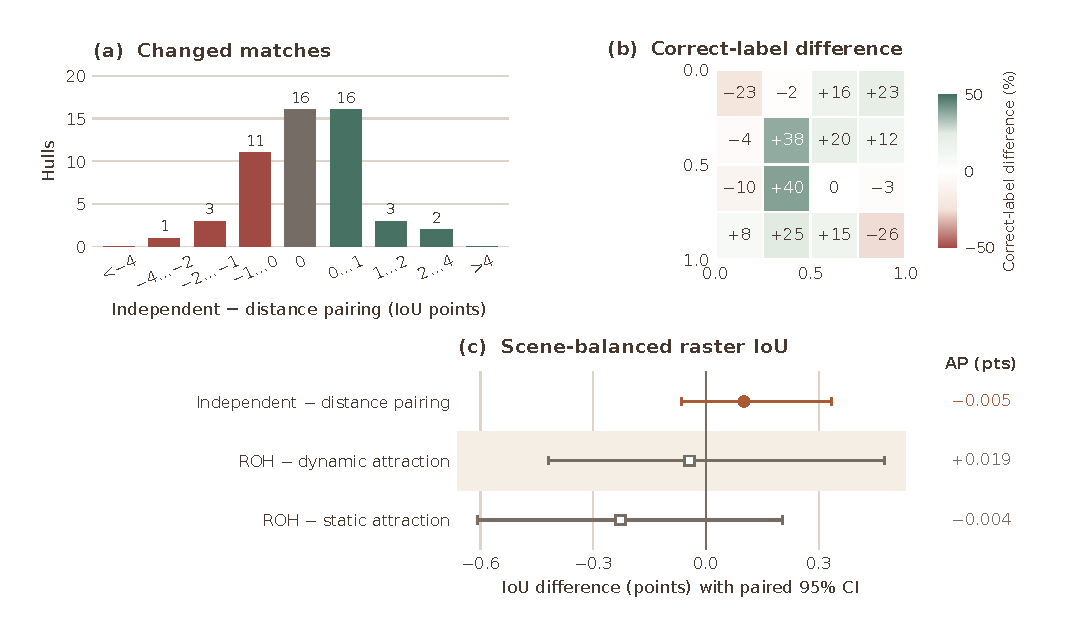
\includegraphics[width=\ifnativecases.92\else.98\fi \linewidth]{figures/journal_20261126/sarssp_public_summary.pdf}
\caption{Independent versus distance-paired selection at equal signed counts on SAR-SSP. (a) IoU changes for the 52 native matches with different edited masks. (b) Differences in correct labels at disagreeing cells, pooled on a $4\times4$ grid in normalized, axis-aligned GT-mask boxes. Each displayed bin contains contributions from at least five hulls. Color saturates at $\pm50\%$. (c) Raster IoU gives equal weight to parent scenes over 139 hulls and assigns zero change to native misses. Intervals are paired 95\% scene intervals. Mask AP includes all 232 chips.}
\label{fig:sar-ssp-cases}
\end{figure*}\par\noindent\hfil\begin{minipage}{.85\linewidth}
In the spatial panel, bins lie in the image-axis-aligned enclosing box of each reference. We report a bin only if at least five hulls contribute. The scene-balanced IoU intervals resample parent scenes.
\end{minipage}\hfil\par
\endgroup
\twocolumn
\section{Full ablations and edit-budget controls}
\label{sec:ablation}
Three ablations distinguish what the occupancy head learns from how its scores are used. The first compares features, supervision and head capacity at common sites. The second holds the signed counts fixed and changes the selection rule on one side at a time. The third holds the whole-mask refiner response fixed and varies writable support, total count and the split between additions and removals.

\subsection{ROH inputs, supervision, and capacity}

A reference-guided upper bound separates restrictions on the choice of cells from errors in their scores. On the 412 detector-visible FIT109 matches, a reference-guided writer reaches IoU 0.90 for 11 hulls under fixed pairing, 27 under independent equal-count selection, and 38 when addition and removal counts can differ. These are conditional ceilings on the original support. With actual point predictions at matched counts, adding partner features or supervising their difference directly offers limited gains. These results motivate the compact ROH.

Our adaptation of Atkinson's attraction rule~\cite{atkinson} uses a five-pixel radius and decay length. At the same 43,624 dynamic swaps on 6,159 FIT109 candidates, ROH, dynamic and static ranking yield AP scores of 53.344, 48.152 and 48.669. Relative to dynamic attraction, ROH ranking gains 1.104 continuous IoU points (\([0.788,1.446]\)) and loses 0.164 AP90 points. Keeping each neighbor's own gray-rank affinity over equal-distance mean affinity gains 1.519 AP points and 0.165 points of reference-normalized intersection (\([0.080,0.264]\)). Endpoint gray rank alone and ROH ranking exceed the aligned-affinity control by 0.370 and 3.039 AP points. The five source-group holdouts apply to the ROH fits. The detector previously trained on FIT109.

On detector-held-out DEV705, the frozen all-FIT109 ROH and the two attraction rules each make 262,802 swaps on 37,811 candidates, covering all 1,447 eligible matches. Their AP scores are 50.727 for ROH ranking, 48.299 for dynamic attraction, and 48.396 for static attraction. Learning gains 5.353 AP75 and 1.150 continuous IoU points relative to dynamic attraction, with a paired 27-prefix 95\% IoU interval of \([0.927,1.397]\). Excluding four empty reference rasters yields a gain of 2.434 AP points.

At fixed counts, the apparent benefit of fractional supervision depends on which binary target replaces it. On D-FINE FIT109, fractional targets gain 0.184 AP and 0.111 IoU points over COCO rasters. The gains over targets thresholded at 0.50 are 0.051 AP and 0.034 IoU points, with a negative AP effect for one fit. Across three fits of the RF-DETR ROH on 74 Instance-RSDD images, full fractions score 0.030 AP and 0.009 IoU points lower than hardening all targets except 0.50, with an IoU interval of \([-0.018,-0.002]\). Against COCO rasters, the same full fractions gain 0.122 AP and 0.109 IoU points. The comparison therefore depends on the alternative representation.

For the capacity comparison, we retrain the scalar ROH and the larger point-head comparator on FIT109 features from frozen RF-DETR~\cite{rfdetr} with center-aligned training masks, using the official implementation (version 1.12.0). The three repetitions share the same detector checkpoint, DEV705 population and 67,386 native mapped candidates. The 1,321-parameter ROH and 139,265-parameter comparator receive the same features and 200 updates per refit. Table~\ref{tab:rfdetr} evaluates COCO mask AP against 1,782 annotations. Continuous IoU uses 1,461 fixed matches with equal weight for each of the 27 source-prefix groups. For paired resampling, we first average the three head results within each group.

\begin{table}[t]
\centering
\caption{RF-DETR DEV705 capacity and write rules. Scores are means of three fits on the 0--100 scale.}
\label{tab:rfdetr}
\footnotesize
\begin{tabular}{@{}lrrr@{}}
\toprule
Mask policy & AP & AP75 & Fixed IoU\\
\midrule
N: Raw RF-DETR & 56.072 & 65.433 & 78.940\\
SF: ROH, fixed pairing & 56.006 & 65.264 & 78.889\\
SU=F: Independent, SF count & 56.912 & 66.844 & 79.528\\
SU: Independent, natural count & 56.865 & 66.785 & 79.537\\
LF=S: Large, fixed, SU count & 55.693 & 64.369 & 78.741\\
LU=S: Large, independent, SU count & 56.860 & 66.925 & 79.530\\
LW=S: Large, free-write, SU count & 56.669 & 66.893 & 79.390\\
NP=S: Native ranks, SU count & 55.935 & 64.767 & 78.786\\
\bottomrule
\end{tabular}
\end{table}

The natural-count ROH writer (SU) gains 0.808, 0.847 and 0.726 AP points over the native detector. Its mean continuous IoU gain is 0.598 points, with a paired source-group 95\% interval of \([0.513,0.698]\). At the ROH's fixed-pair count, SU=F exceeds SF by 0.906 AP and 0.639 IoU points, with an IoU interval of \([0.548,0.743]\). Comparing SU with the larger free writer LW=S at the same count gives smaller gains of 0.197 AP and 0.147 IoU points. The IoU interval is \([-0.041,0.415]\), and neither point estimate reaches the prespecified 0.30 AP and 0.20 IoU margins for advancing that comparison. With the large head and count held fixed, independent LU=S gains 0.192 AP and 0.139 continuous IoU points over LW=S.

At the 0.90 IoU threshold, 9, 9 and 10 of the 86 native matches above the threshold fall to or below it across the three ROH fits. In the opposite direction, 29, 21 and 18 matches cross upward. The effects apply to the shared frozen detector and point-head training budget. They support relaxing the fixed pairing under this configuration, with the effect of conserving area relative to a competitive point writer still uncertain.

At the realized SU counts of each ROH fit, ranking by true pixel occupancy would add 2.111 continuous IoU points over SU, with a paired interval of \([1.863,2.383]\). Allowing the addition and removal counts to vary at the same total would add another 1.001 points, with interval \([0.814,1.224]\). With learned ranks held fixed, a quota-only oracle gains 1.264 points over SU. All three ceilings retain the 1,461 native matches and the original endpoint support.

At matched FIT109 counts, query-conditioned features gain 0.352 AP and 0.073 IoU points over the ordinary feature control. The IoU interval spans zero. Zero padding and within-candidate permutation both achieve higher AP than the query-conditioned features.

In the five source-group-held-out FIT109 PointRend folds, each head receives 200 updates. The learned full paste raises AP by 2.440 points relative to the coarse paste and remains 3.851 points below the native mask. At matched counts, balanced independent editing gains 1.047 AP and 0.262 IoU points over fixed pairing, with interval \([0.131,0.406]\). Relative to unconstrained-area editing, the gains are 0.938 AP and 0.084 IoU points, with interval \([-0.039,0.202]\). Here the detector has seen the FIT images.

On HRSID FIT36, five registered shift views retain the original queries, native support, 166 fixed matches and 1,209 swaps. Ranking on the second-worst signed score loses 0.333 continuous IoU points to ranking by the mean logit (\([-0.489,-0.149]\)).

\subsection{Independent selection on the addition and removal sides}
\label{sec:side-ablation}

An equal-count exchange can improve the addition, the removal, or both. We form four masks from the same sampled endpoints and ROH scores. In the baseline mask, both sides follow fixed pairing. The next two masks use independent ranks on either the addition or the removal side while retaining the fixed locations on the other side. Both sides are independent in the final mask. The original detection score and the same addition count, removal count and foreground area carry through all four rules. The intervention separates the decisions in Eq.~\eqref{eq:independent-estimated-gain}. For any fixed hull, each side contributes additively to \(g\) in Eq.~\eqref{eq:intersect-changes}. Mask AP can also reflect interactions from matching across the ranked detection list.

\begin{table*}[t]
\centering
\caption{Instance-RSDD signed-side ablation at matched counts. The 42-chip view is nested.}
\label{tab:signed-side-ablation}
\footnotesize
\setlength{\tabcolsep}{5pt}
\begin{tabular}{@{}llrrrr@{}}
\toprule
View & ROH fit & Both fixed & Independent add only & Independent remove only & Both independent\\
\midrule
Gaofen-3, 583 chips & H1 & 61.036 & 61.331 & 61.286 & \textbf{61.518}\\
Gaofen-3, 583 chips & H2 & 60.984 & 61.207 & 61.302 & \textbf{61.468}\\
Reserve, 74 chips & H1 & 58.278 & 58.545 & 58.426 & \textbf{58.714}\\
Date-separated, 42 chips & H1 & 61.283 & 61.769 & 61.698 & \textbf{62.123}\\
\bottomrule
\end{tabular}
\end{table*}

\begin{figure}[t]
\centering
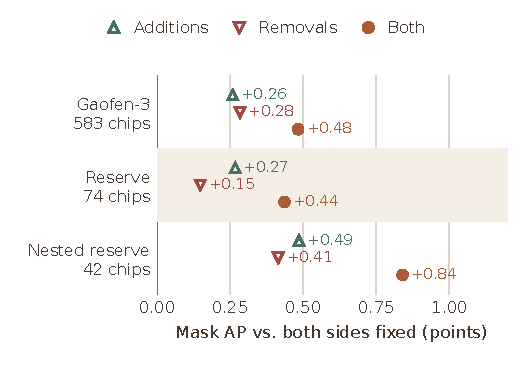
\includegraphics[width=\columnwidth]{figures/journal_20261126/independent_sides_ablation.pdf}
\caption{Change in mask AP when independent ranking selects additions, removals or both, at equal signed counts. Gaofen-3 values average two frozen ROH fits.}
\label{fig:signed-side-ablation}
\end{figure}

Switching either side raises AP in Table~\ref{tab:signed-side-ablation} and Fig.~\ref{fig:signed-side-ablation}. Using independent ranks on both sides attains the highest measured AP in each row. It also improves fixed-match continuous IoU over each single-side rule on the main Gaofen-3 and reserve views. The AP interaction is small and changes sign across cohorts. The size of each side's contribution therefore depends on the cohort and metric.

With the ROH and counts fixed, freeing both sides adds 0.224 AP and 0.175 IoU points over freeing only the additions on Gaofen-3 (means over two ROH fits, \([0.130,0.222]\)). On the 74 chips, the corresponding gains are 0.169 AP and 0.170 IoU points (\([0.108,0.251]\)). Relative to independent deletions alone, the gains are 0.199 AP and 0.085 IoU points (\([0.049,0.120]\)) and 0.288 AP and 0.148 IoU points (\([0.042,0.252]\)), respectively. AP increases for both Gaofen-3 heads and in the reserve. Both IoU intervals are also positive in the date-separated view.

At the dynamic-attraction budget, learned addition and removal locations increase DEV705 intersection by \(+0.308\) and \(+0.446\) points of hull area, respectively. Both reduce intersection on PSeg-SSDD and UEIKAP342. On those external cohorts, the interval for the difference between the two sides spans zero. A \href{https://github.com/bingzhi495-creator/SAR-SEAL-research/blob/3f8f738/research_round_20260925_global/ATTRACTION_LOCAL_CORRECTION_ACTUAL_20261123.md}{ridge adjudicator} fitted on 4,063 disputed FIT109 pairs gains 0.018 IoU points over using the scores alone on DEV705 (\([0.008,0.028]\)). On deduplicated PSeg, its IoU interval spans zero and static attraction leads by 0.115 AP points.

A second score field tests whether the same pairing effect recurs with a frozen Phoenix refiner. At matched counts, independent selection exceeds fixed pairing by 0.486 AP and 0.327 continuous IoU points on Instance-RSDD and by 0.731 AP and 0.595 IoU points on PSeg-SSDD. Optimizing the pairing under the original per-candidate maximum swap distance accounts for 0.250 and 0.534 AP points of those differences. Removing that cap adds 0.236 and 0.197 AP points, below the 0.30-point margin on both full cohorts. The corresponding IoU increments are 0.197 (\([0.063,0.324]\)) and 0.280 (\([0.171,0.398]\)) points. On PSeg, static attraction still leads the independent arm by 0.195 AP points at that count.

\subsection{Writable support, edit count, and signed allocation}

\begin{table*}[t]
\centering
\caption{Writable support and count for a frozen Phoenix response (points). The balanced condition retains narrow support and the same total.}
\label{tab:phoenix-factors}
\footnotesize
\setlength{\tabcolsep}{5pt}
\begin{tabular}{@{}llrrr@{\quad}rrr@{}}
\toprule
 & & \multicolumn{3}{c}{Instance-RSDD reserve (74)} & \multicolumn{3}{c}{PSeg-SSDD official (232)}\\
\cmidrule(lr){3-5}\cmidrule(l){6-8}
Support & Writing rule & Flips & AP & IoU & Flips & AP & IoU\\
\midrule
Whole grid & Phoenix threshold & 2,042,908 & 49.085 & 69.428 & 3,391,327 & 13.922 & 65.739\\
Whole grid & Count, free split & 59,800 & 58.478 & 78.890 & 147,540 & 16.447 & 69.741\\
Narrow & Phoenix threshold & 114,328 & 58.498 & 79.260 & 270,637 & 15.866 & 68.996\\
Narrow & Count, free split & 59,800 & 58.787 & 79.171 & 147,540 & 16.380 & 69.417\\
Narrow & Count, equal signs & 59,800 & 58.976 & 79.253 & 147,540 & 18.222 & 70.568\\
\bottomrule
\end{tabular}
\end{table*}

Table~\ref{tab:phoenix-factors} gives the effects of writable support, count and split for a fixed Phoenix response. To isolate area conservation, we keep the Phoenix probabilities, sampled endpoints and \(2k\) flips per candidate unchanged. For a frozen occupancy \(p\), we rank additions by \(p-0.50\) and removals by \(0.50-p\). Within each quota, the sorted prefixes maximize the estimated gain in pixel correctness. With \(d\) unrestricted, 59,800 flips add a net 23,828 foreground cells across the Instance-RSDD reserve predictions. Strict balance gains 0.190 AP and 0.083 continuous IoU points over free allocation, with interval \([-0.191,0.401]\). The written masks differ for 45 fixed hulls across 11 sensor--date blocks. Allowing \(|d|\) up to two cells gives 58.856 AP, between 58.976 for strict balance and 58.787 for free allocation. All three retain the 81 original matches. In a single HRSID DEV705 fit with a source-trained ROH at 631,020 fixed flips, free allocation leads balance by 0.212 AP and 0.009 continuous IoU points. Strict balance has a small, uncertain IoU advantage on the reserve. Free allocation leads on DEV705 with a different ranking field. The larger degradation under whole-grid writing motivates a separate support and count comparison.

For the Instance-RSDD support and count comparison, we use the same fifth-iteration Phoenix posterior for each of the 4,107 positive-budget candidates. Other candidates retain their native masks. The narrow writer edits the original sampled endpoints. The whole-grid writer can edit the original image grid. The threshold rule applies the Phoenix binary output at each eligible cell. The exact-count rule keeps the original narrow-run \(2k\) budget and chooses the signed split that maximizes the sum of estimated pixel-correctness gains. Reapplying the narrow exact-count and whole-grid threshold rules reproduces the original masks for all 4,107 candidates, and all 259,242 recorded probabilities match.

\begin{figure*}[t]
\centering
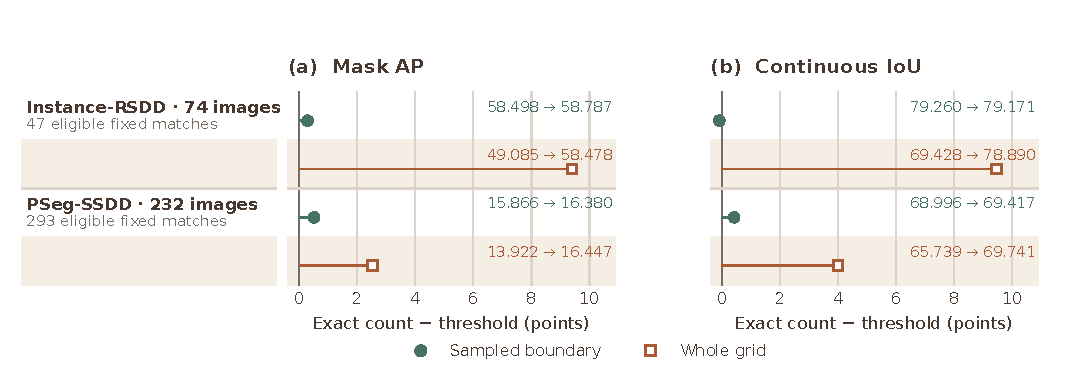
\includegraphics[width=\textwidth]{figures/journal_20261126/phoenix_budget_by_dataset.pdf}
\caption{Exact-count minus threshold effects for narrow and whole-grid support with the same frozen Phoenix response. Numeric labels give the two original scores. Continuous IoU uses 47 fixed matches on Instance-RSDD and 293 on PSeg-SSDD.}
\label{fig:phoenix-support-budget}
\end{figure*}

On the Instance-RSDD reserve, applying the original count across the whole grid cuts the edits from 2,042,908 to 59,800 and raises AP from 49.085 to 58.478 (Fig.~\ref{fig:phoenix-support-budget}). Fixed continuous IoU gains 9.462 points, with a paired 95\% interval of \([6.329,13.283]\). False-positive area falls by 33.131 points of reference area (\([-49.245,-19.298]\)), while missed area changes by \(+2.957\) points (\([-0.058,5.863]\)). Rematching at IoU 0.50 recovers from 77 to 81 hulls. The exact-count policy still writes 44,158 cells outside the sampled support. Its AP remains 0.201 points above native, with AR100 0.494 points lower.

On the narrow support, applying the same count rule changes AP by \(+0.289\) points and IoU by \(-0.089\) points. The whole-support effect thus exceeds the narrow-support effect by 9.105 AP and 9.551 continuous IoU points, with a paired IoU interval of \([6.398,13.365]\). At the same exact count, narrowing the support gives \(+0.309\) AP and \(+0.281\) IoU points relative to the whole-grid writer, with interval \([-0.025,0.666]\). The whole-grid count effect stays positive on the nested 42-chip date-separated view at 12.920 AP and 10.672 IoU points.

For PSeg-SSDD we use frozen D-FINE and keep the original dynamic-attraction counts for the 11,054 editable candidates. The whole-grid threshold rule writes 3,391,327 cells. At the same support, imposing the count reduces that total to 147,540 and raises AP from 13.922 to 16.447. Fixed continuous IoU gains 4.001 points (\([2.644,5.382]\)). Foreground outside the reference falls by 7.382 points of reference area (\([-11.989,-3.621]\)). Rematching at IoU 0.50 covers 404 hulls after the cap, down from 407, while the number retaining the original candidate rises from 377 to 394. On the 222-image view excluding exact historical fitting overlaps, AP and continuous IoU gains are 2.694 and 4.095 points. Every comparison includes the full original candidate stream for the applicable images in the official allocation.

On narrow PSeg support, the exact-count rule gains 0.514 AP and 0.422 IoU points over narrow thresholding (\([0.253,0.595]\)). Comparing narrow and whole-grid writing at the same exact count gives the narrow writer 0.067 lower AP and 0.323 lower IoU points (\([-0.560,-0.111]\)). The whole-grid count effect exceeds the narrow-support count effect by 2.011 AP and 3.580 IoU points, with an IoU interval of \([2.316,4.887]\). Across both datasets, the budget constraint reduces the harm of whole-grid thresholding. The effects of restricting support at that budget differ by dataset. On PSeg-SSDD, the whole-grid exact-count Phoenix arm remains 1.528 AP points below native D-FINE and 1.970 points below matched static attraction.

At the same 147,540 narrow-support flips, allocating half to additions and half to removals raises PSeg Phoenix AP from 16.380 to 18.222 and continuous IoU by 1.151 points (\([0.701,1.594]\)). The two masks differ for 283 of 293 fixed matches across 137 of 143 decoded-image groups. Missed area falls by 1.428 points of reference area and false-positive area rises by 0.340 points. The balanced writer trails matched static attraction by 0.195 AP and 0.076 IoU points (\([-0.246,0.105]\)). It also scores 0.109 AP points below the matched learned head, with a 0.186-point IoU advantage (\([0.036,0.339]\)). After excluding ten exact historical overlaps, balance gains 2.093 AP and 1.232 IoU points over free allocation (\([0.762,1.682]\)). Its differences relative to the two matched ranking methods retain their directions.

\section{Coverage, topology, physical interpretation and computation}
An edit can improve overlap only if the relevant hull cells are accessible and their occupancy scores distinguish missed foreground from excess foreground. When the original mask area is wrong, the split between additions and removals also matters. These conditions explain why transfer performance must be interpreted alongside proposal coverage, reference agreement and the allowed edits.
\subsection{Transfer and reference dependence}
The AP effect of location selection varies across cohorts and references. Both Gaofen-3 detector fits gain AP, while the changes on PSeg-SSDD and SAR-SSP are small. On the same 232 SSDD images, the area-preserving natural-count writer has opposite AP effects under the PSeg and SPSD references. Most of the resulting IoU shift comes from edits at cells the two outlines label differently (Fig.~\ref{fig:reference-disagreement}).

The HRSID official split and SAR-SSP validation set have prior evaluation exposure. The Gaofen-3 fits share target scenes, and the reserve views are distinguished by parent IDs and sensor--date keys (Table~\ref{tab:cohorts}). Independent reference scoring remains pending for the frozen outputs on 12 prospective Umbra windows and a separate 24-collect cohort.

\subsection{Proposal coverage and edit constraints}
A reference-guided ceiling identifies which misses can be recovered from the existing candidates and their allowed edit regions. On SAR-SSP, only one of the 47 unmatched hulls can cross mask IoU 0.50 under reference-guided edits within the original support and exchange cap. The 164 raw queries add box-level coverage for two of those 47 hulls. If arbitrary reference-guided edits are allowed inside the existing boxes, nine hulls can be recovered at fixed area and another 19 when the area is allowed to change. These are per-hull ceilings that allow candidate reuse. The 92 original matches admit a different test. At their observed endpoint counts, reference-optimal edits can improve scene-balanced discrete IoU by 1.187 points over learned independence and by 0.895 points over reference-optimal distance pairing. The matched cases leave room for better local ranking. Many misses would require wider support or different proposals. On UEIKAP, only 17 of 139 released hulls have native matches with a positive edit budget.

The stock SegRefiner tests distinguish deletion locations from deletion count. With the original additions and the same number of deletions, replacing the deleted cells by reference-guided choices gains 5.594 and 3.512 IoU points on the evaluated Instance-RSDD and PSeg-SSDD matches, respectively. Allowing fewer deletions adds 4.256 and 4.189 points. We also tried a rule without reference labels that caps deletions at the smaller of the stock addition and deletion counts. Uniform selection under this cap gains 0.907 and 0.878 AP points over stock. The addition-only and local ROH writers still score higher on both cohorts. A suitable count can recover part of the loss while leaving substantial error in the choice of cells.

\subsection{Topology and physical interpretation}

Contour regularity is a separate property from area and overlap. Pairing constrains endpoint distance, while the balanced split fixes the number of foreground cells. SharpContour parameterizes the outline directly, and DSR-Net models structural relations within the detector~\cite{sharpcontour,dsr}. The present writer isolates the effects of position and count. Its topology is assessed from the resulting masks.
Even a single area-preserving exchange can split a connected component, open a hole or extend the mask toward a neighboring vessel. Natural-count selection increased the number of holes in 1,544 of 10,466 edited PSeg masks. The same number of edits ranked by the native response increased holes in 519 masks. Yet 24 of the 26 Instance-RSDD hulls harmed by stock SegRefiner deletion kept the same number of components and holes. Those counts can stay constant when a narrow edge or an end is misplaced. At the small-size limit, all 107 nonempty candidate masks in the Schwegmann set~\cite{schwegmann} fell below the 32-cell area floor.

The physical-length comparison covers fewer ships. Of the 142 NovaSAR AIS chips~\cite{nastar}, 34 yielded common mask spans and 17 admitted positive-budget edits. Equal-count independent selection changed absolute length error by \(+0.204\)~m (\([-0.110,0.581]\)~m). On 25 common Sentinel-1A cases from the Gulf data~\cite{gulf}, the nominal mean absolute error changed by \(-0.168\)~m (\([-1.523,1.692]\)~m). Using AIS headings in a 23-case sensitivity analysis still left a mean geolocated length excess of 71.27~m. With these coverage and uncertainty limits, the mask-overlap gains establish little about physical length accuracy.

\subsection{Computation and repeatability}
The timing comparisons depend on which inputs are already available. The D-FINE CUDA detector and postprocessor took 11.74\,s for 232 PSeg images. With the detector outputs already in memory, interpolation that gives the same outputs reduced single-thread local refinement from 158.8 to 104.3\,ms/image. Across two single-thread passes on the 74 Instance-RSDD chips, ROH writing took 227.1\,ms/image, the equal-count PointRend adaptation took 1,221.5\,ms/image, and whole-RoI PointRend took 1,049.2\,ms/image. The adaptation renders the whole region of interest before the constrained write. In a separate six-pass test with the endpoints, occupancy scores, counts and initial pairings already cached, distance-first, bounded and independent selection took 26.1, 138.6 and 27.4\,ms/image, respectively, including RLE encoding on the same logical CPU.

Frozen Phoenix took 1,404.48\,s on PSeg with four two-thread CPU workers, five iterations and 11,054 prompts. Stock SegRefiner-LR took 454.18\,s for 74 Instance-RSDD images on an RTX 3090 Ti and 13,420.42\,s on PSeg under shared workstation load. 

Independent reevaluation reproduced 3,434 table entries for the HRSID official and Instance-RSDD 740 allocations, and 1,470 for the first RF-DETR pipeline on the 74-chip reserve.

\IEEEtriggeratref{4}
\begin{thebibliography}{20}
\bibitem{dfine} A. Saakyan and D. Solntsev, ``D-FINE-seg: Object detection and instance segmentation framework with multi-backend deployment,'' \href{https://arxiv.org/abs/2602.23043}{arXiv:2602.23043}, 2026.
\bibitem{rfdetr} I. Robinson, P. Robicheaux, M. Popov, D. Ramanan, and N. Peri, ``RF-DETR: Neural architecture search for real-time detection transformers,'' in \emph{Proc. Int. Conf. Learn. Represent. (ICLR)}, 2026.
\bibitem{phoenix} B. Kim and S. J. Hwang, ``Learning from adversity: Semantic-aware mask refinement through adversarial perturbation,'' in \emph{Proc. Eur. Conf. Comput. Vis. (ECCV)}, 2026, pp. 75--92. \href{https://doi.org/10.1007/978-3-032-37520-9_5}{10.1007/978-3-032-37520-9\_5}.
\bibitem{rankrma} Z. Wang and B. Dai, ``RankSEG-RMA: An efficient segmentation algorithm via reciprocal moment approximation,'' in \emph{Adv. Neural Inf. Process. Syst.}, vol. 38, 2025. \href{https://doi.org/10.52202/085713-5452}{10.52202/085713-5452}.
\bibitem{rankseg} B. Dai and C. Li, ``RankSEG: A consistent ranking-based framework for segmentation,'' \emph{J. Mach. Learn. Res.}, vol. 24, no. 224, pp. 1--50, \href{https://www.jmlr.org/papers/v24/22-0712.html}{2023}.
\bibitem{atkinson} P. M. Atkinson, ``Sub-pixel target mapping from soft-classified, remotely sensed imagery,'' \emph{Photogramm. Eng. Remote Sens.}, vol. 71, no. 7, pp. 839--846, 2005. \href{https://doi.org/10.14358/PERS.71.7.839}{10.14358/PERS.71.7.839}.
\bibitem{hrsid} S. Wei, X. Zeng, Q. Qu, M. Wang, H. Su, and J. Shi, ``HRSID: A high-resolution SAR images dataset for ship detection and instance segmentation,'' \emph{IEEE Access}, vol. 8, pp. 120234--120254, \href{https://doi.org/10.1109/ACCESS.2020.3005861}{2020}.
\bibitem{rsdd} X. Yang, Q. Zhang, Q. Dong, Z. Han, X. Luo, and D. Wei, ``Ship instance segmentation based on rotated bounding boxes for SAR images,'' \emph{Remote Sens.}, vol. 15, no. 5, Art. no. 1324, \href{https://doi.org/10.3390/rs15051324}{2023}.
\bibitem{ssdd} T. Zhang \emph{et al.}, ``SAR Ship Detection Dataset (SSDD): Official release and comprehensive data analysis,'' \emph{Remote Sens.}, vol. 13, no. 18, Art. no. 3690, 2021. \href{https://doi.org/10.3390/rs13183690}{10.3390/rs13183690}.
\bibitem{slgsea} R. Deng, T. Zhang, G. Gao, L. Zhang, S. Wei, and X. Zhang, ``SLGSea: Spatialized language guidance with scattering-aware query construction for ship--sea--land panoptic segmentation in SAR imagery,'' project repository and dataset release. \href{https://github.com/deng1218/SLGSea}{Code and data}.
\bibitem{boundaryiou} B. Cheng, R. Girshick, P. Doll{\'a}r, A. C. Berg, and A. Kirillov, ``Boundary IoU: Improving object-centric image segmentation evaluation,'' in \emph{Proc. IEEE/CVF Conf. Comput. Vis. Pattern Recognit. (CVPR)}, 2021. \href{https://arxiv.org/abs/2103.16562}{arXiv:2103.16562}.
\bibitem{rsddsar} C. Xu \emph{et al.}, ``RSDD-SAR: Rotated ship detection dataset in SAR images,'' \emph{J. Radars}, vol. 11, no. 4, pp. 581--599, 2022. \href{https://doi.org/10.12000/JR22007}{10.12000/JR22007}.
\bibitem{rankdep} Z. Wang and B. Dai, ``On the relaxation of conditional independence assumption for image segmentation,'' \href{https://arxiv.org/abs/2609.38930}{arXiv:2609.38930}, 2026.
\bibitem{ueikap} A. Mazzeo \emph{et al.}, ``UEIKAP dataset,'' Zenodo, ver. 1.0, \href{https://doi.org/10.5281/zenodo.18391027}{2026}.
\bibitem{airsarship} X. Sun, Z. Wang, Y. Sun, W. Diao, Y. Zhang, and K. Fu, ``AIR-SARShip-1.0: High-resolution SAR ship detection dataset,'' \emph{J. Radars}, vol. 8, no. 6, pp. 852--862, 2019. \href{https://doi.org/10.12000/JR19097}{10.12000/JR19097}.
\bibitem{sharpcontour} C. Zhu, X. Zhang, Y. Li, L. Qiu, K. Han, and X. Han, ``SharpContour: A contour-based boundary refinement approach for efficient and accurate instance segmentation,'' in \emph{Proc. IEEE/CVF Conf. Comput. Vis. Pattern Recognit. (CVPR)}, 2022, pp. 4392--4401.
\bibitem{dsr} S.-W. He, W. Xiong, and L.-B. Yao, ``SAR ship instance segmentation method in complex scenes jointly driven by differential physical fields and structured graph reasoning,'' \emph{Acta Electronica Sinica}, pp. 1--11, 2026. \href{https://doi.org/10.12263/DZXB.20260699}{10.12263/DZXB.20260699}.
\bibitem{schwegmann} C. P. Schwegmann, W. Kleynhans, B. P. Salmon, L. W. Mdakane, and R. G. V. Meyer, ``Very deep learning for ship discrimination in Synthetic Aperture Radar imagery,'' in \emph{Proc. IEEE Int. Geosci. Remote Sens. Symp. (IGARSS)}, 2016, pp. 104--107. \href{https://doi.org/10.1109/IGARSS.2016.7729017}{10.1109/IGARSS.2016.7729017}.
\bibitem{nastar} B. Hosseiny, K. Kamirul, O. Pappas, and A. Achim, ``NASTaR: A NovaSAR-based automated ship target recognition dataset,'' \emph{IEEE Geosci. Remote Sens. Lett.}, vol. 23, Art. no. 1502605, 2026. \href{https://doi.org/10.1109/LGRS.2026.3679941}{10.1109/LGRS.2026.3679941}.
\bibitem{gulf} M. Shaya, ``SAR Ship Gulf: Sentinel-1 GRD ship chips with AIS labels,'' Zenodo, ver. 1, 2026. \href{https://doi.org/10.5281/zenodo.21000650}{10.5281/zenodo.21000650}.
\end{thebibliography}
\end{document}
